\section{Chapter introduction}

Considering its impacts on the energy budget at the surface, the effects of irrigation follow a marked diurnal cycle, with distinct effects in nighttime and daytime and varying amplitude depending on insolation. Average monthly or seasonal studies (like the works presented in Chapter \ref{chap:monthly}) cannot allow a detailed analysis of these impacts, and simulation outputs at a finer temporal resolution must be used.

Although it's based on the same simulation setup as Chapter \ref{chap:monthly}, this chapter focuses on the month on July 2021, and on part of the Ebro Valley. This study area and period were selected to include the measurement sites and special observation period (SOP) of the LIAISE field campaign. This enables direct comparison to local observations of temperature, humidity, wind and turbulent fluxes on irrigated and rainfed sites, at the surface and in the boundary layer. Furthermore, several modelling experiments were conducted over this area and period, in particular using the mesoscale MesoNH model at 2-km resolution. These simulations served as an intermediate between punctual observations and the regional climate model, bringing new perspective on the following questions:

\begin{itemize}
    \item How does the ICOLMDZOR-LAM perform over the LIAISE study area, relative to observations and mesoscale simulations?
    \item To what extent does simulated irrigation improve the performance of the LAM? What limits its ability to reproduce observations on irrigated and rainfed sites at the diurnal scale?
    \item Are the effects of simulated irrigation limited to surface variables or do they propagate to the vertical structure of the ABL? 
    \item Are the effects of simulated irrigation only visible over the irrigated areas or do they also affect neighbouring rainfed areas?
    \item Over such a heterogeneous terrain, how can representativity of the LAM be defined and to what extent is it achieved?
\end{itemize}

\section{The LIAISE field campaign}
%objectives
%period
%sites
%measurements / instruments
%irrigation practices and timing. Urgell canal adduction
%overview of synoptic conditions, rainfall
% simulation experiment with conceptual and mesoscale models
%main outcomes so far : Mangan, Lunel (2 sites), Lunel Marinada, intermodel comparison

\section{Simulation experiments}

Several simulations are compared to analyse the diurnal cycle of land-atmosphere coupling variables in the Ebro Valley.
First, the two simulations studied in Section \ref{sec:article1} (\noirr and \irr) were analysed and compared to LIAISE observations using hourly outputs over the month of July 2021.

Then, sensitivity experiments were conducted to increase irrigation over grid cell corresponding to the irrigated site of La Cendrosa, leading to the simulation henceforth referred to as \irrboost. This simulation was only run over the month of July, starting from the same state as \noirr and \irr on July 1st 2021, and involved significant changes in both on the computation of irrigation demand, and on the water availability. 
Regarding demand, the irrigated fraction was slightly increased to make sure that all of the soiltile dedicated to low vegetation and crops was considered as irrigated land. This soiltile represents 83.5\% of the grid cell, the rest being occupied by trees (12.4\%) and bare soil (4.1\%). This fraction was also reduced to 0\% on the Els Plans site to make sure there would be no irrigation demand computed in this grid cell.
More importantly, the \betairrig parameter, which had been set to 0.6 after the offline calibration in Chapter \ref{routing} to avoid excessive depletion of the groundwater and river reservoirs, was increased to 1. This means that the irrigation scheme is aiming to maintain soil moisture in the root zone (first 64cm of soil) to field capacity, making sure that plants would not be limited in their growth by available soil moisture. 
Regarding available water, since this was a short simulation run (one month), very large amounts of water were added in the three routing reservoirs at the simulation initial state, making virtually inifinite amounts of water available for irrigation in the LIAISE region. Obviously, this method is not realistic, nor applicable to longer climate runs, and was only used to test the limits of the irrigation scheme and explore the sensitivities of land-atmosphere interactions in a context where irrigation would be driven by the water demand rather than the supply. 
When comparing to reality, this can also be seen as a way to compensate for the absence of water adduction in the ICOLMDZOR-LAM simulations, a practice that is determinant in the actual supply of irrigated water in the area. %todo:see if this explained in previous sec, refer to it
%todo:see also if irrigation simulation method used by tanguy has been detailed (because that's what it does too)

The three ICOLMDZOR-LAM simulations (\noirr, \irr, \irrboost) are compared to observations and to the MesoNH simulation from July 15th to July 31st. This covers all the LIAISE SOP and allows for the stabilization of irrigation volumes in the \irrboost simulation, since no long-term spinup was conducted with this setup.

%todo:mesoNH (if not presented in previous section ?)
%todo:choice of grid cell -> figure


\section{Surface variables at La Cendrosa and Els Plans}

%cendrosa turbulent fluxes
\begin{figure}[hbtp]
    \centering
    \begin{tabular}{cc}
        \begin{subfigure}[t]{0.5\textwidth}
            \caption{}
            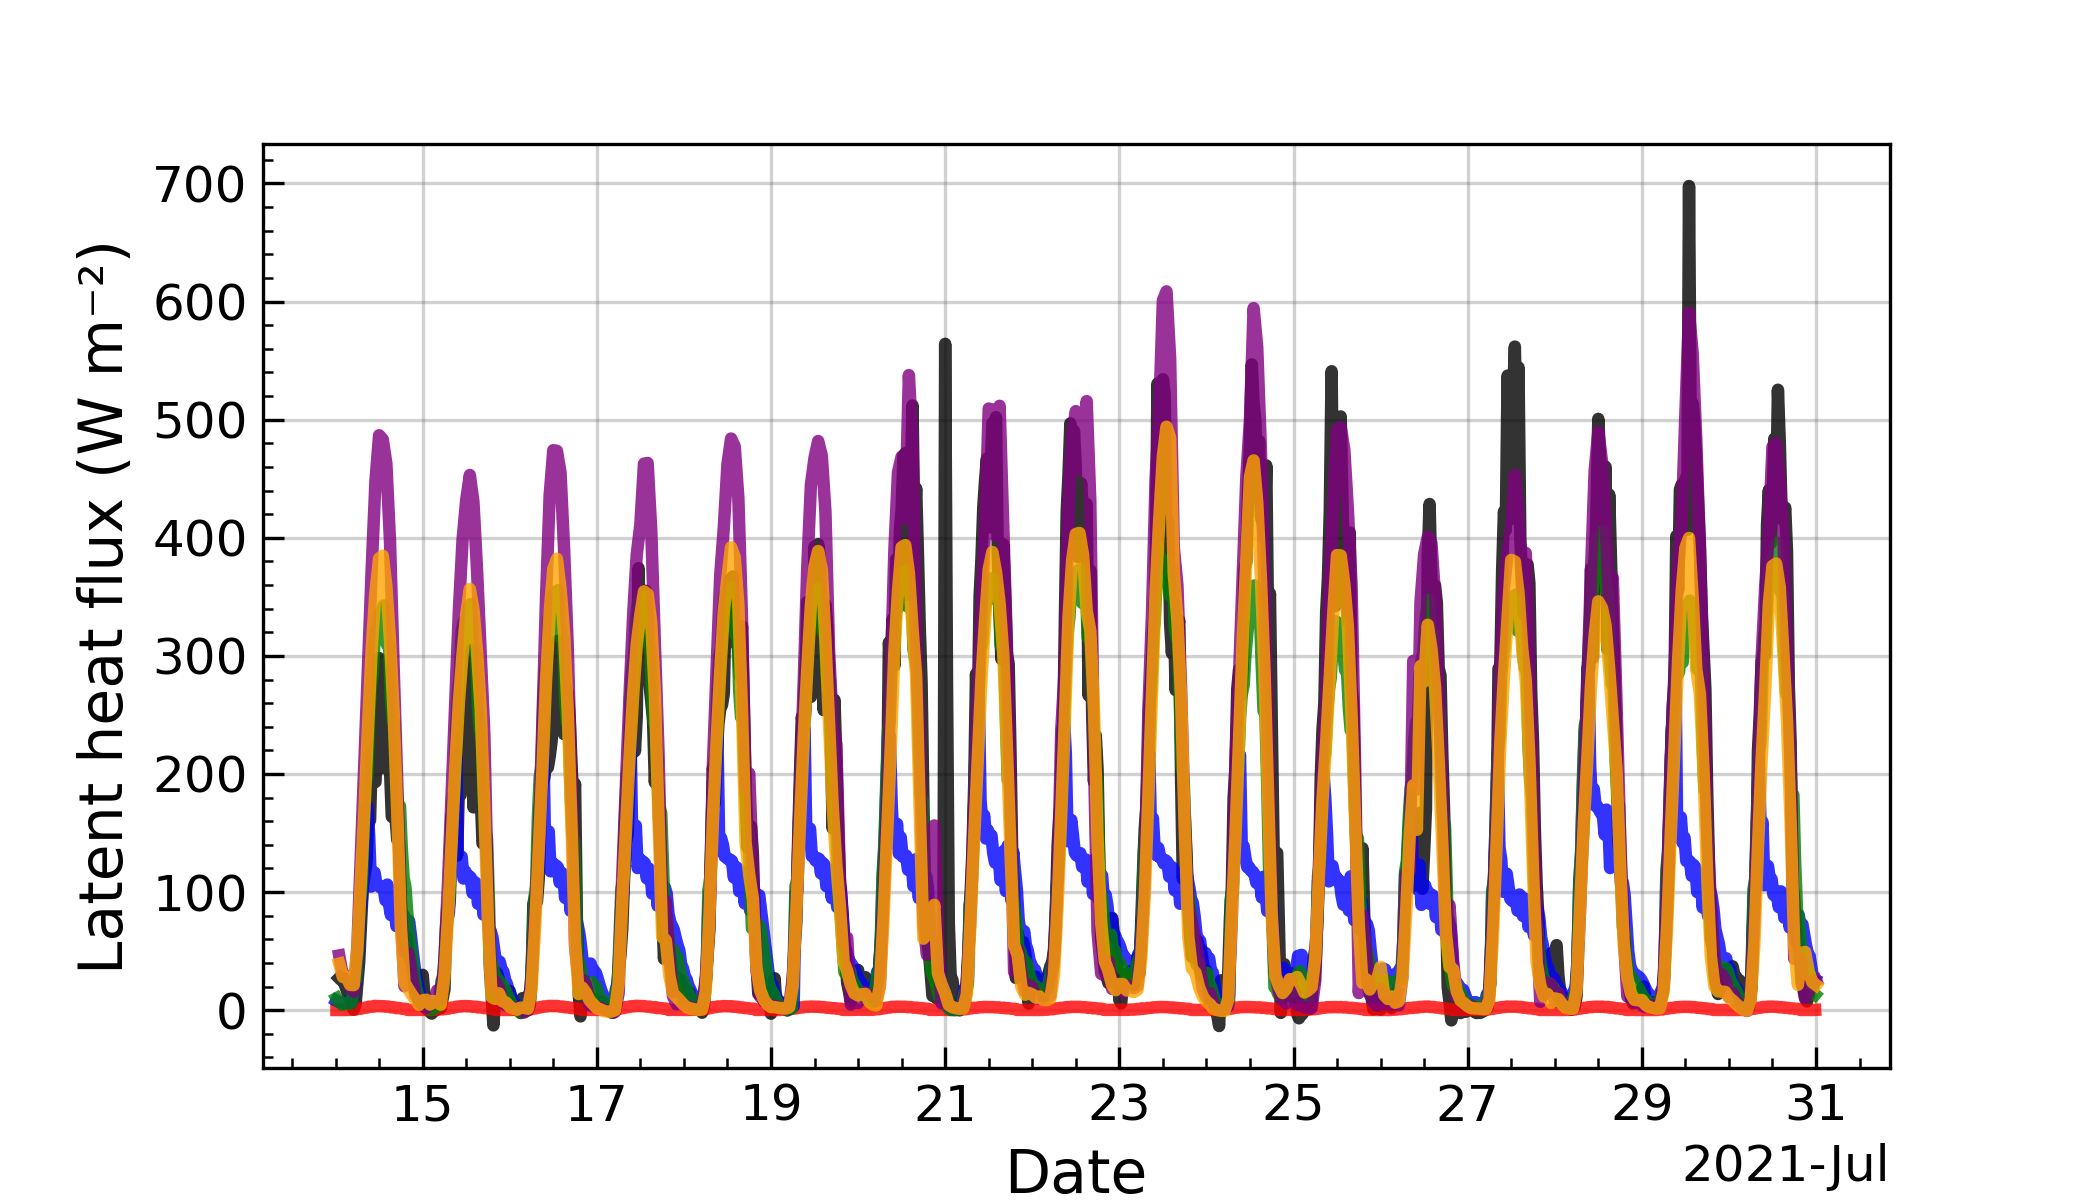
\includegraphics[width=\textwidth]{images/chap5/time_series_cendrosa_flat.png}
        \end{subfigure} &
        \begin{subfigure}[t]{0.5\textwidth}
            \caption{}
            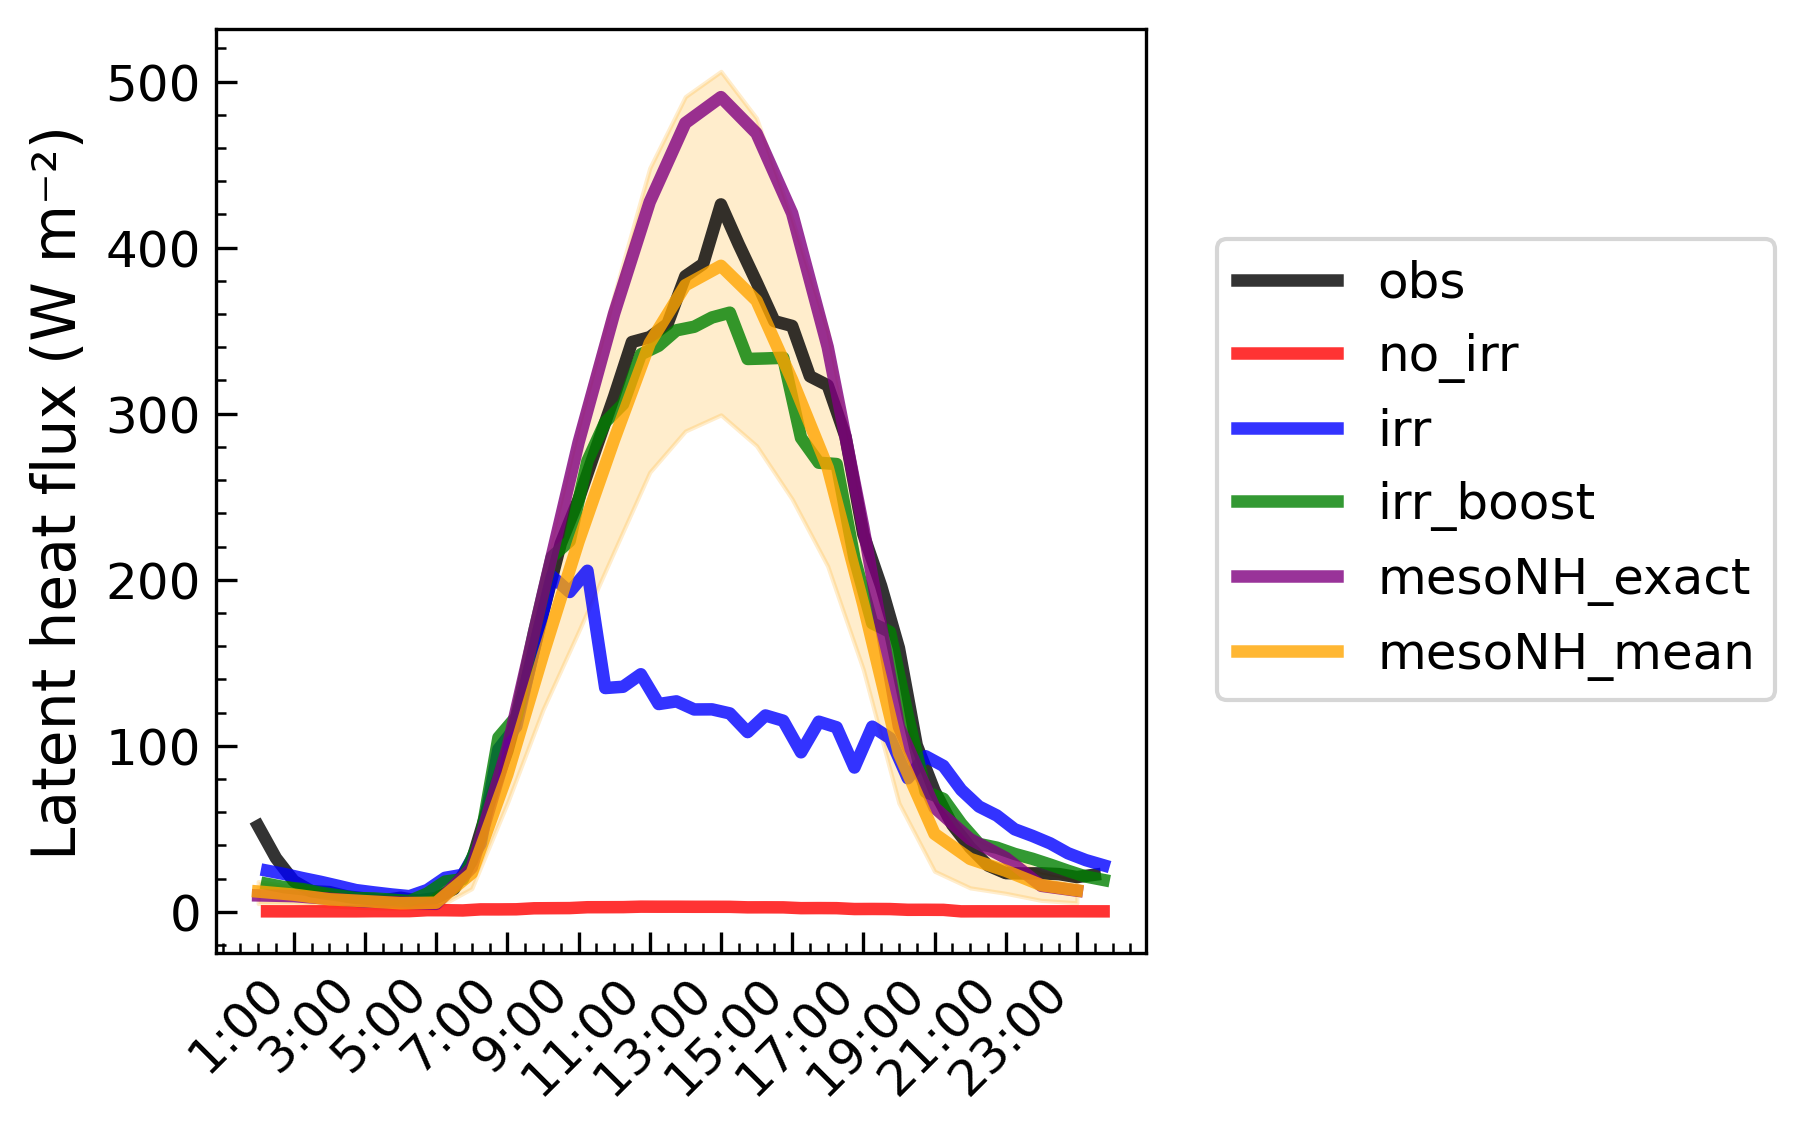
\includegraphics[width=\textwidth]{images/chap5/diurnal_cycle_cendrosa_flat.png}
        \end{subfigure} \\
        
        \vspace{1em} % Add vertical space between the rows

        \begin{subfigure}[t]{0.5\textwidth}
            \caption{}
            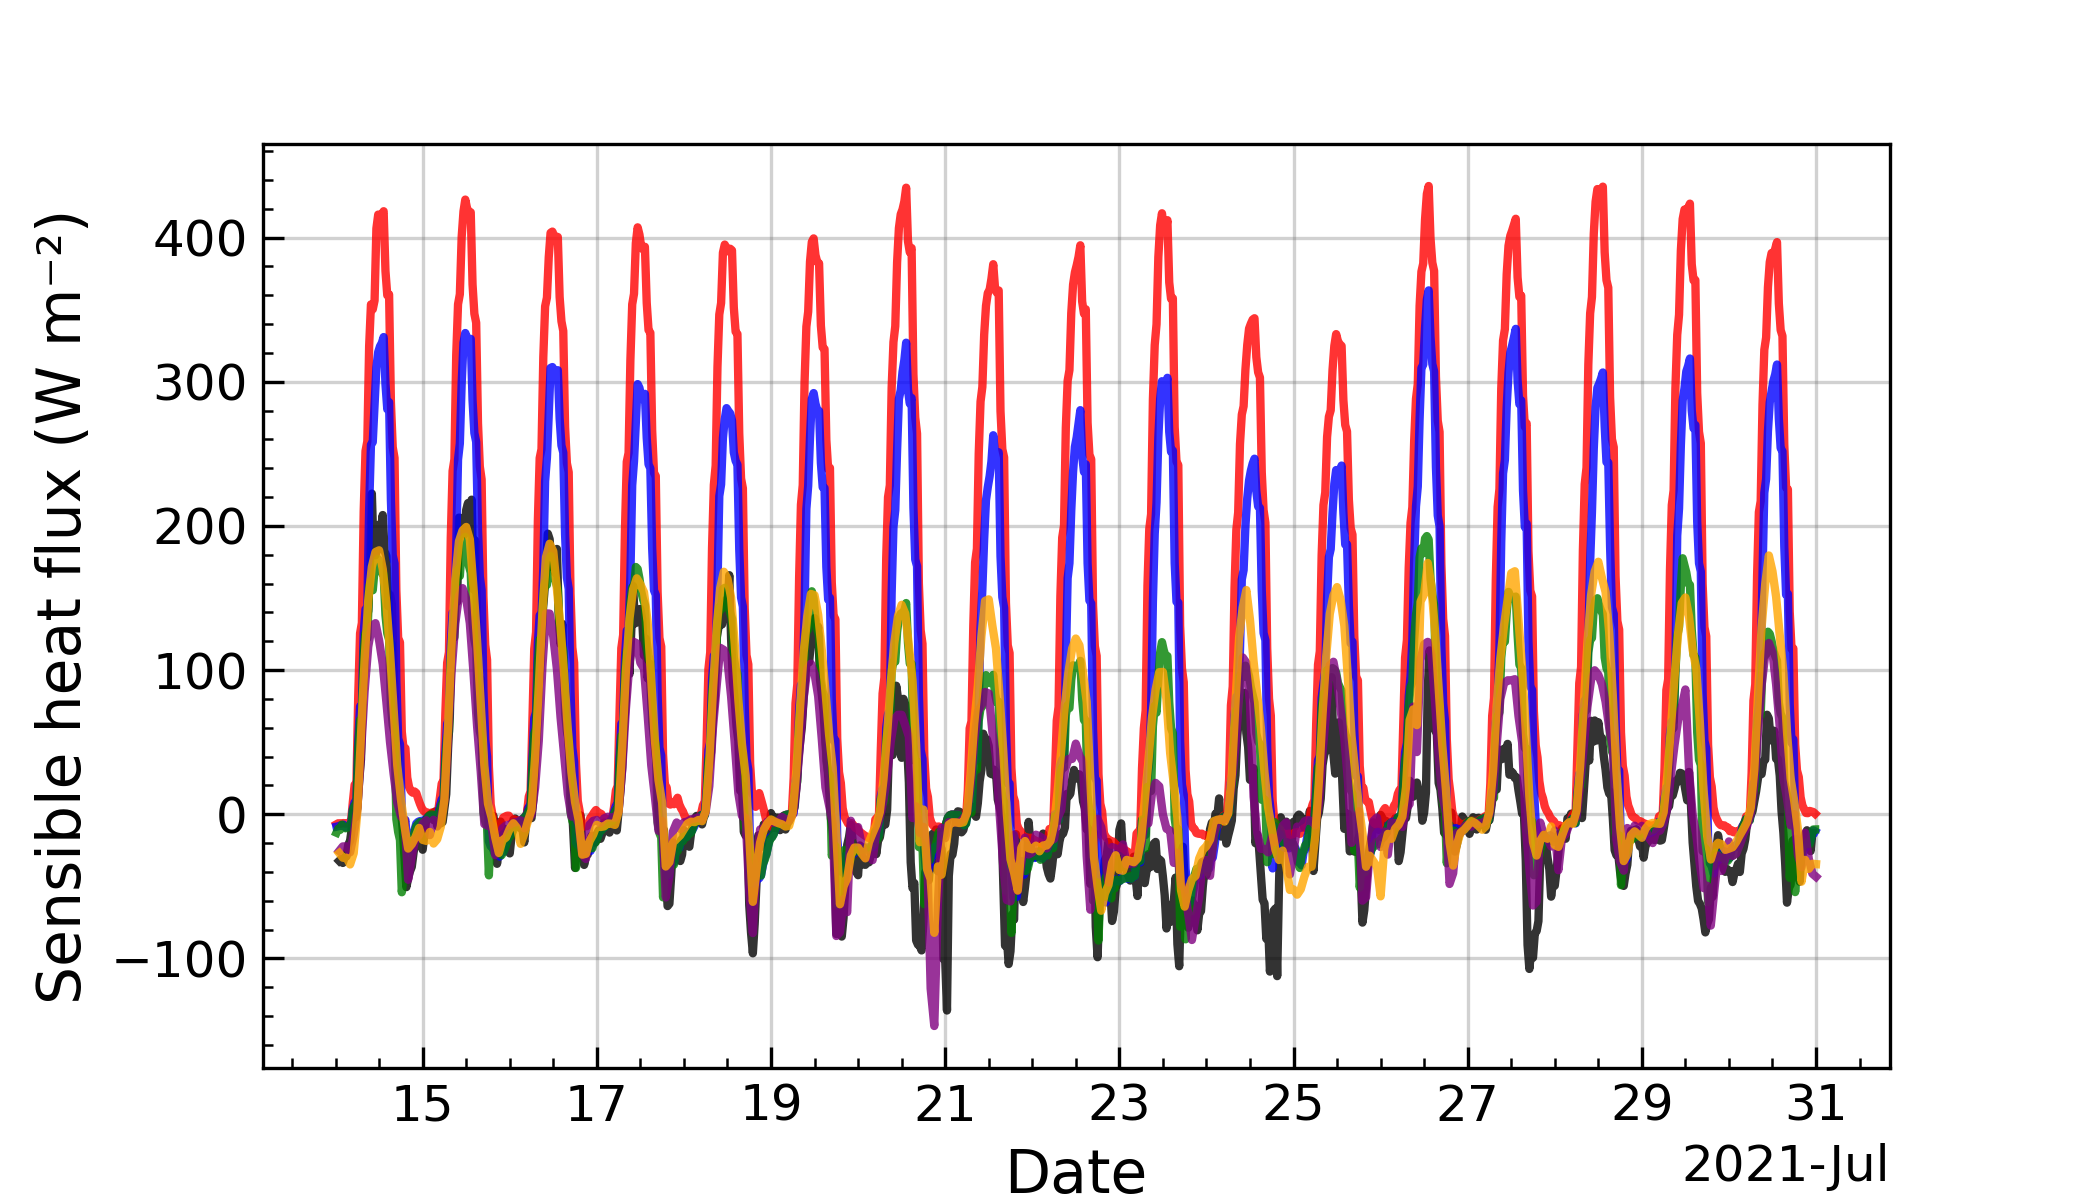
\includegraphics[width=\textwidth]{images/chap5/time_series_cendrosa_sens.png}
        \end{subfigure} &
        \begin{subfigure}[t]{0.5\textwidth}
            \caption{}
            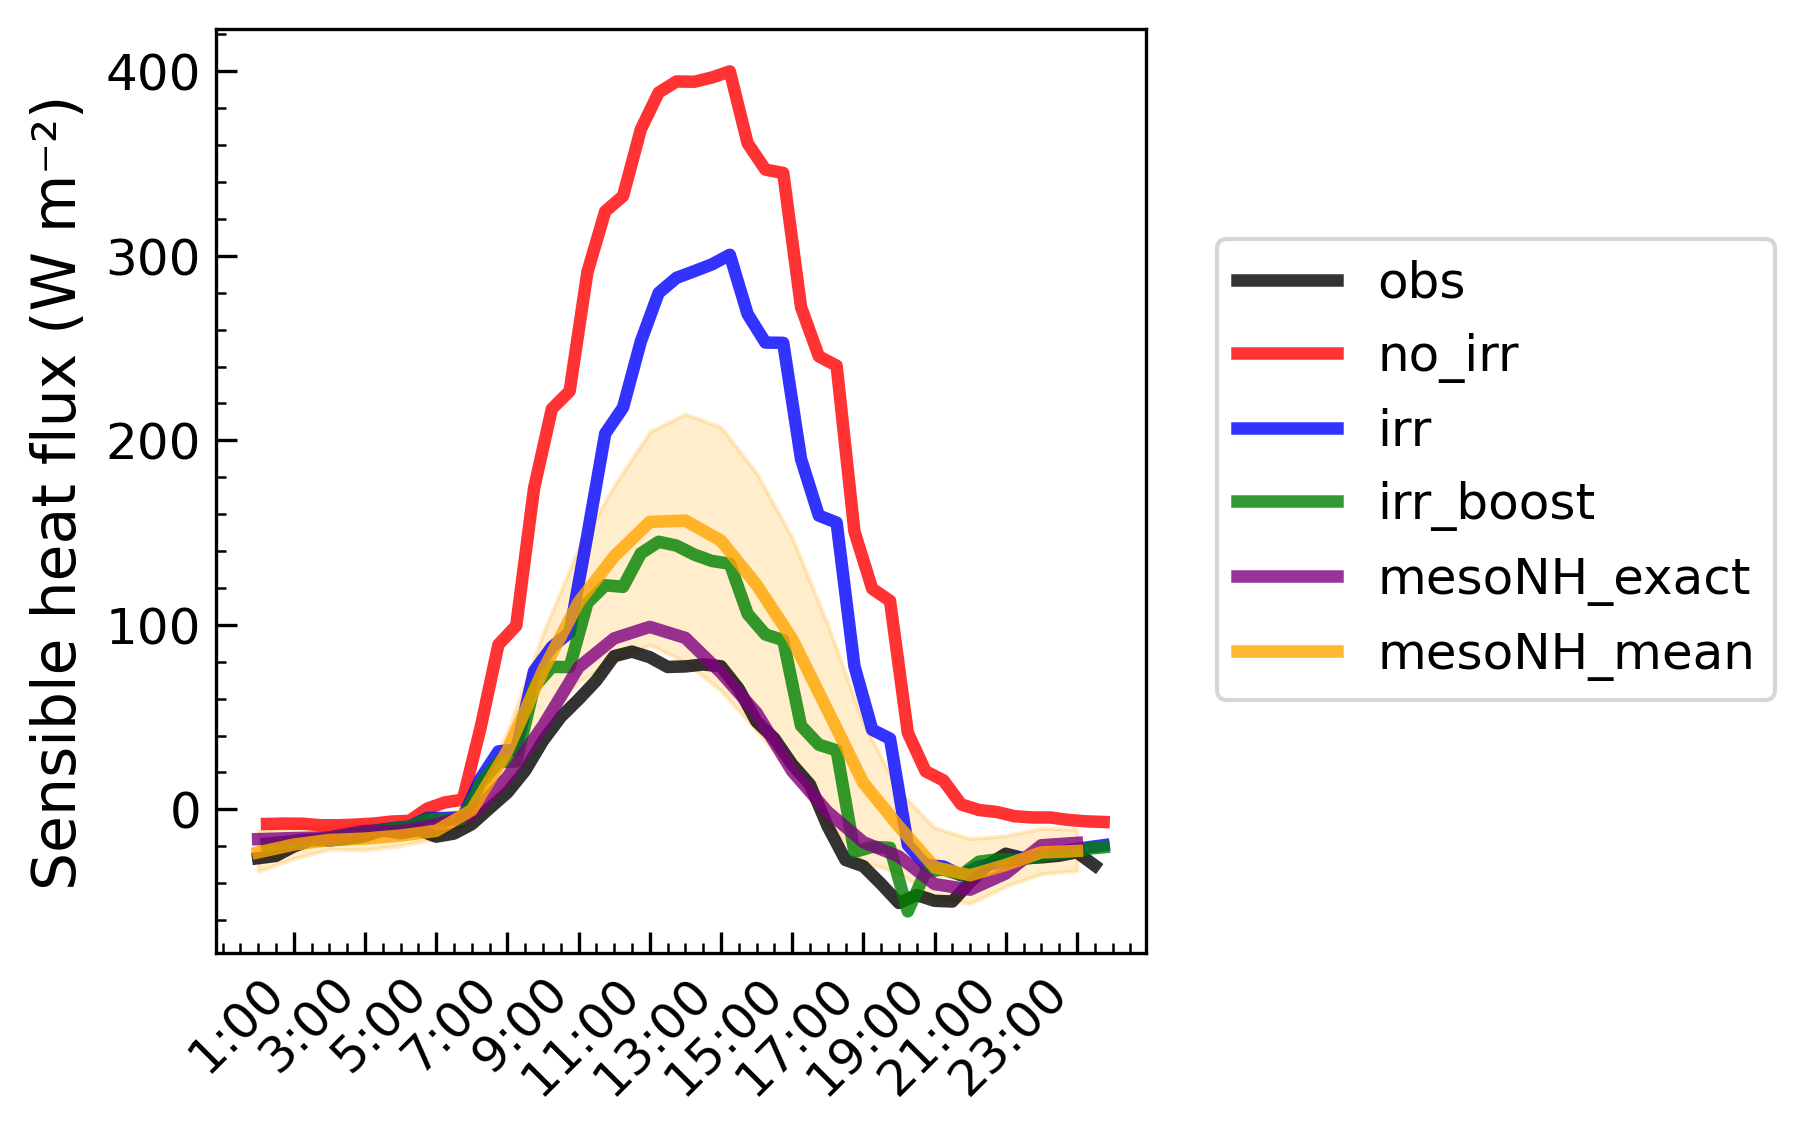
\includegraphics[width=\textwidth]{images/chap5/diurnal_cycle_cendrosa_sens.png}
        \end{subfigure} \\
    \end{tabular}
    \caption{Time series and mean diurnal cycle of surface turbulent fluxes at La Cendrosa (irrigated site), July 15-31 2021.}
\end{figure}

%Els Plans turbulent fluxes
\begin{figure}[hbtp]
    \centering
    \begin{tabular}{cc}
        \begin{subfigure}[t]{0.5\textwidth}
            \caption{}
            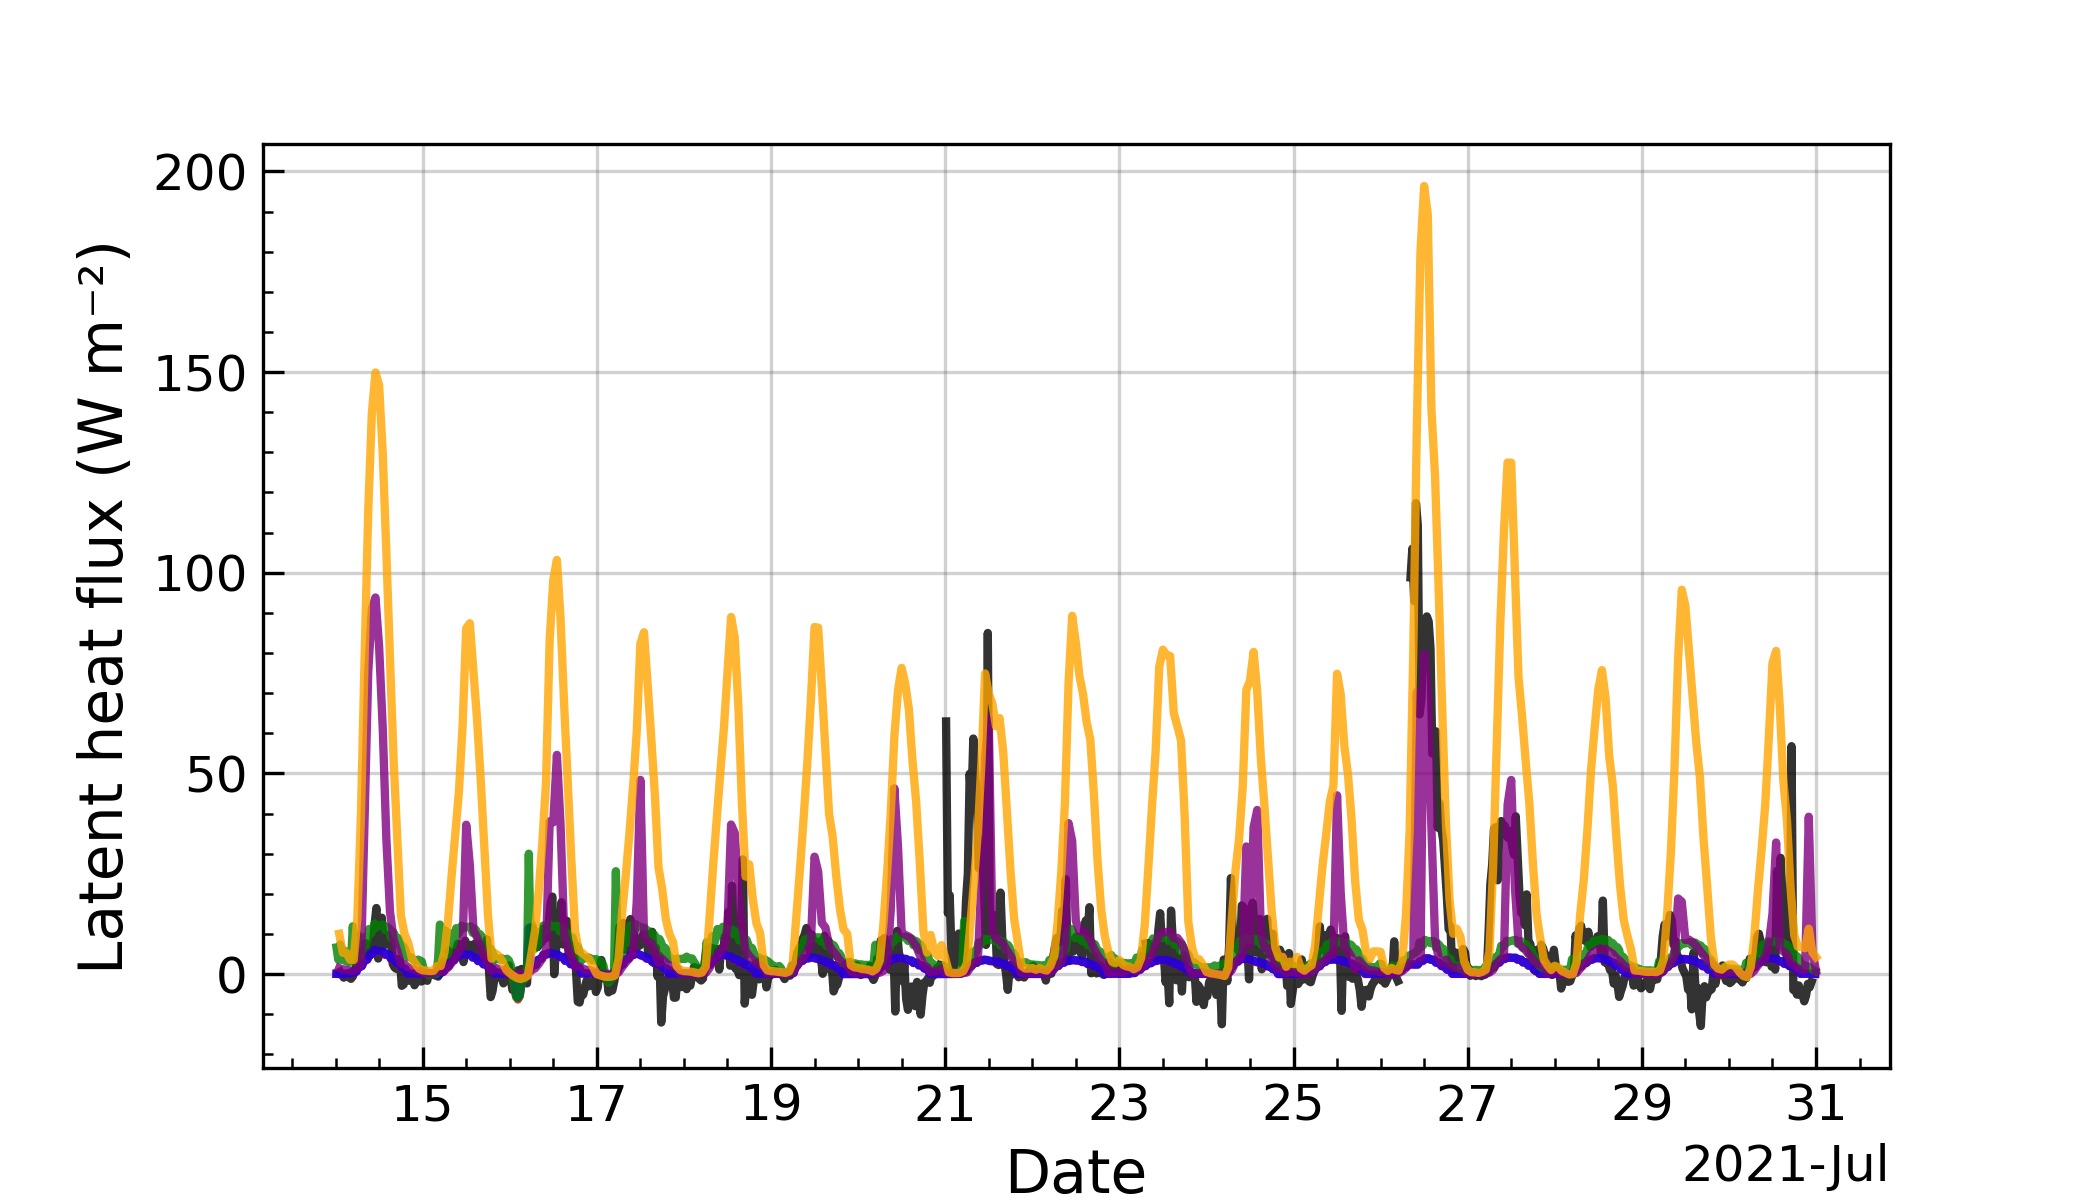
\includegraphics[width=\textwidth]{images/chap5/time_series_elsplans_flat.png}
        \end{subfigure} &
        \begin{subfigure}[t]{0.5\textwidth}
            \caption{}
            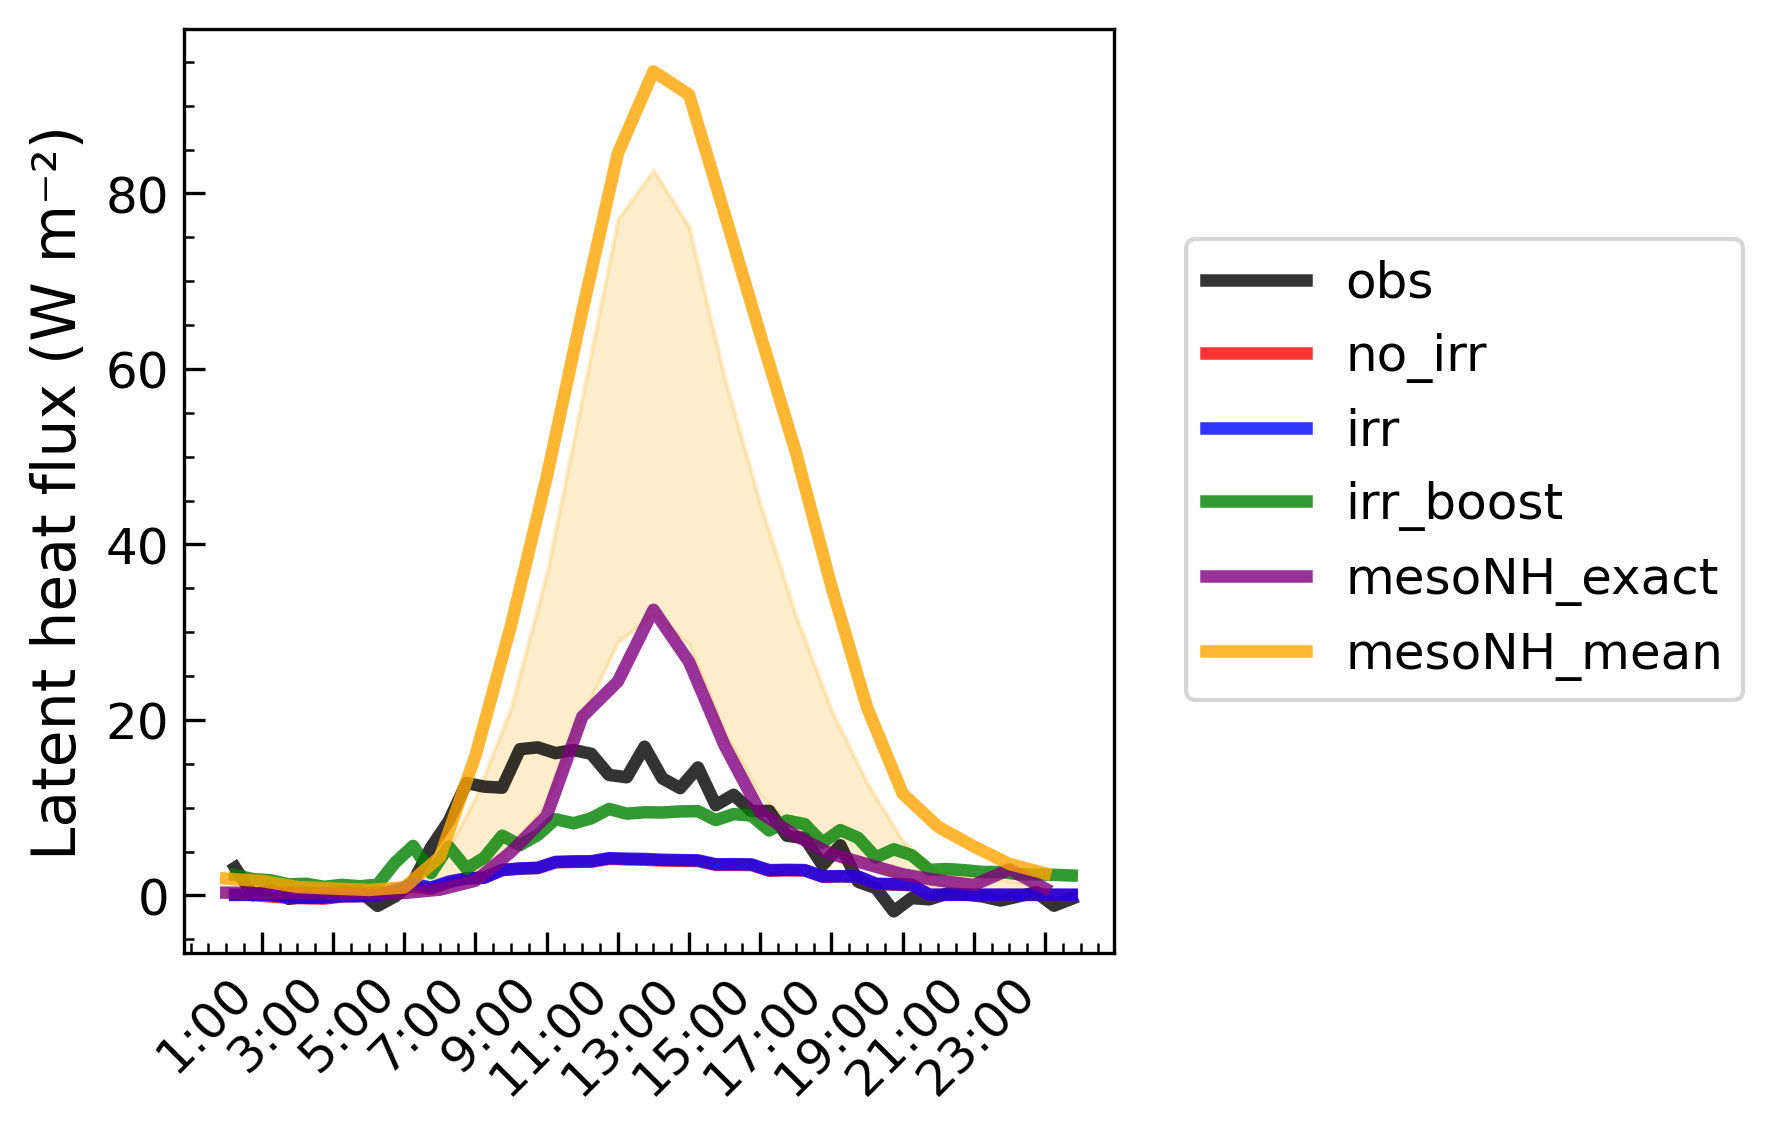
\includegraphics[width=\textwidth]{images/chap5/diurnal_cycle_elsplans_flat.png}
        \end{subfigure} \\
        
        \vspace{1em} % Add vertical space between the rows

        \begin{subfigure}[t]{0.5\textwidth}
            \caption{}
            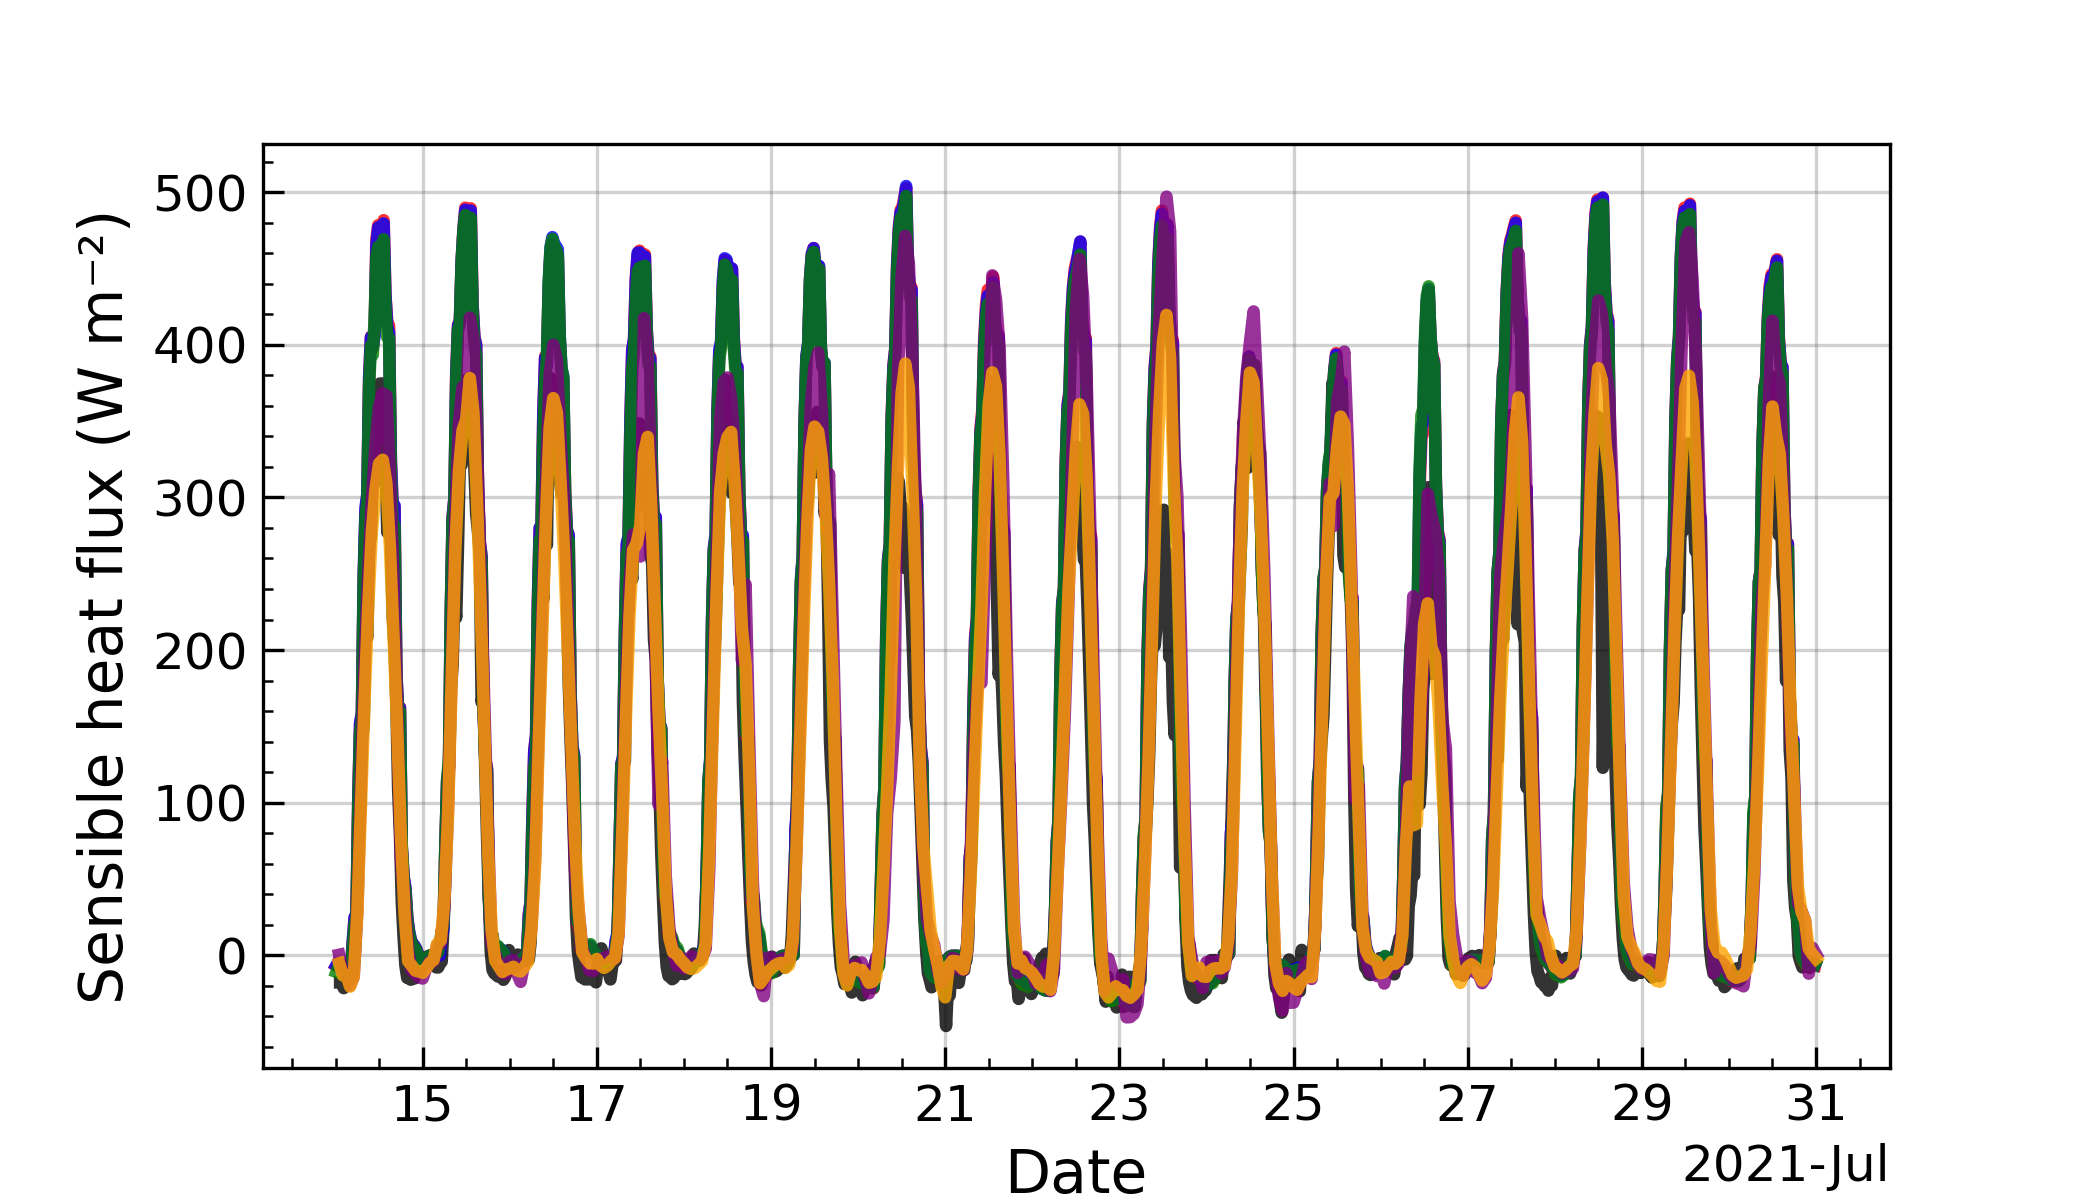
\includegraphics[width=\textwidth]{images/chap5/time_series_elsplans_sens.png}
        \end{subfigure} &
        \begin{subfigure}[t]{0.5\textwidth}
            \caption{}
            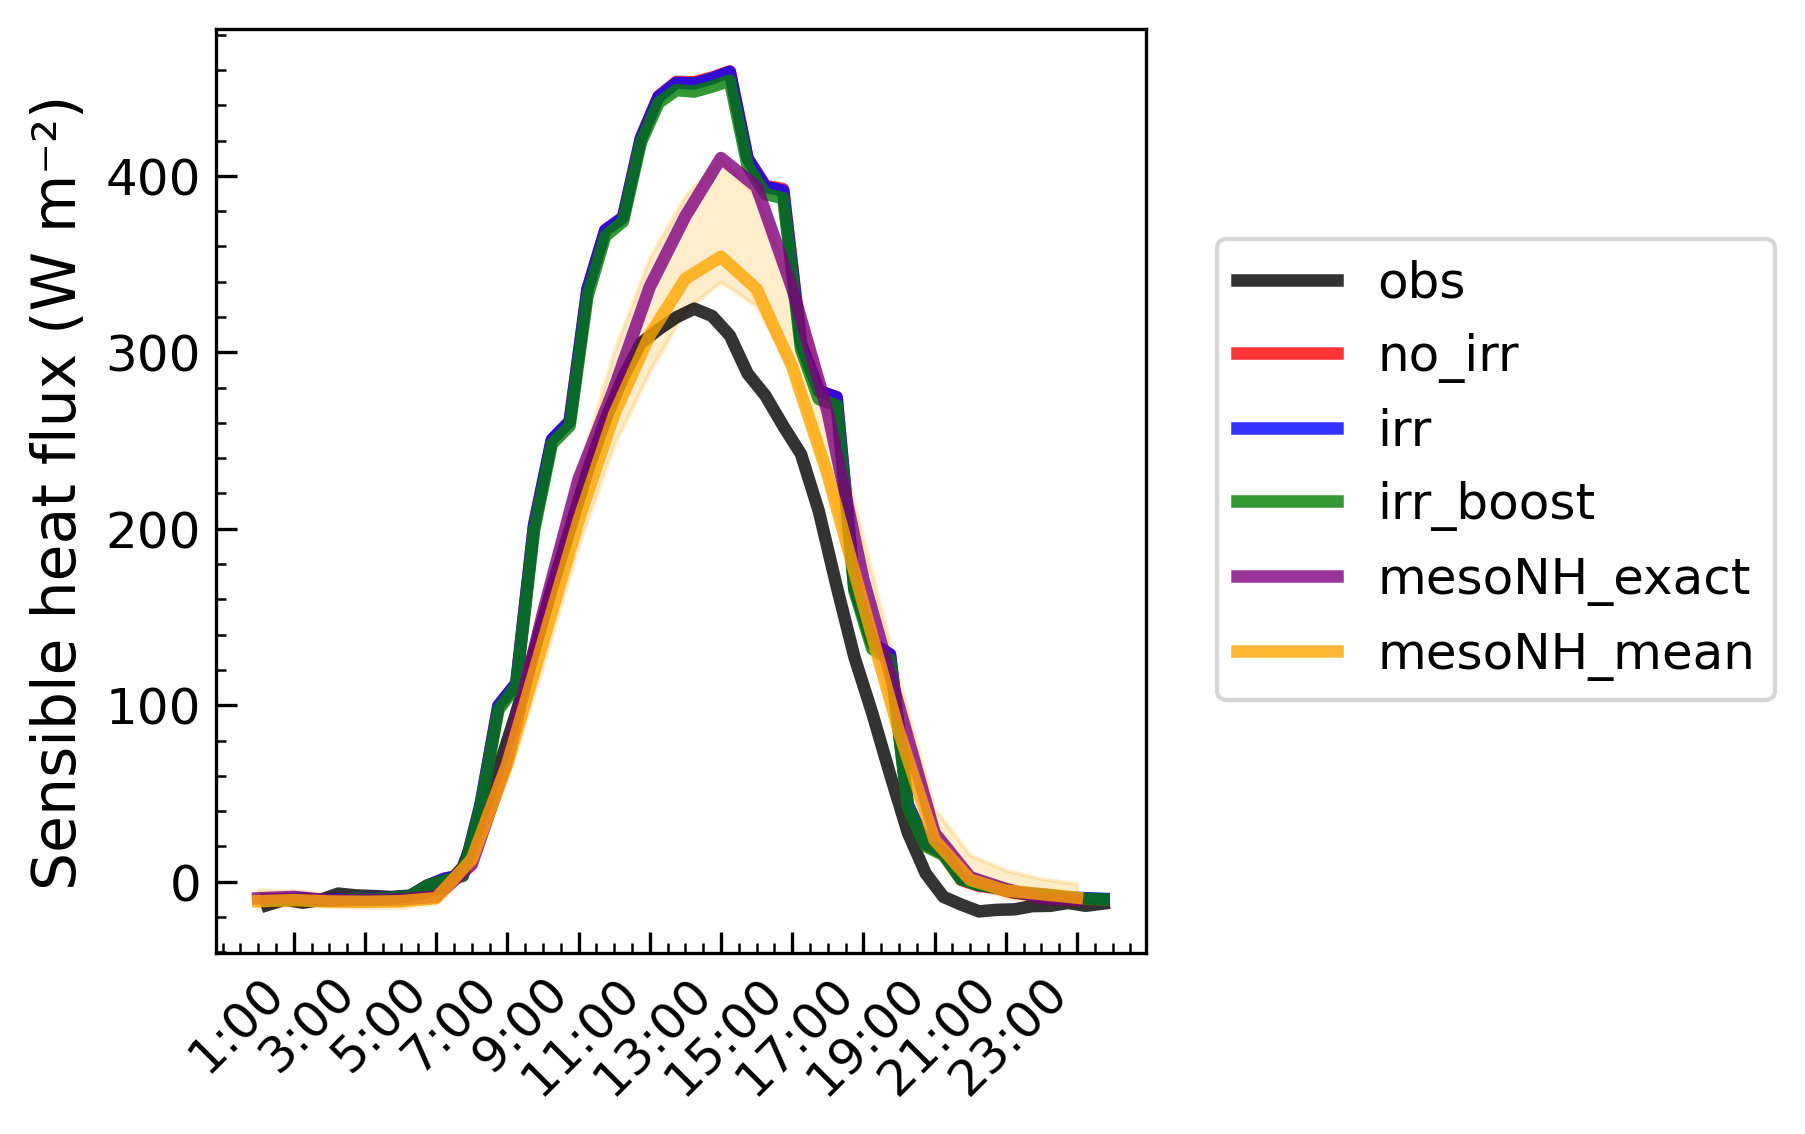
\includegraphics[width=\textwidth]{images/chap5/diurnal_cycle_elsplans_sens.png}
        \end{subfigure} \\
    \end{tabular}
    \caption{Time series and mean diurnal cycle of surface turbulent fluxes at Els Plans (rainfed site), July 15-31 2021.}
\end{figure}


%cendrosa t2m, q2m
\begin{figure}[hbtp]
    \centering
    \begin{tabular}{cc}
        \begin{subfigure}[t]{0.5\textwidth}
            \caption{}
            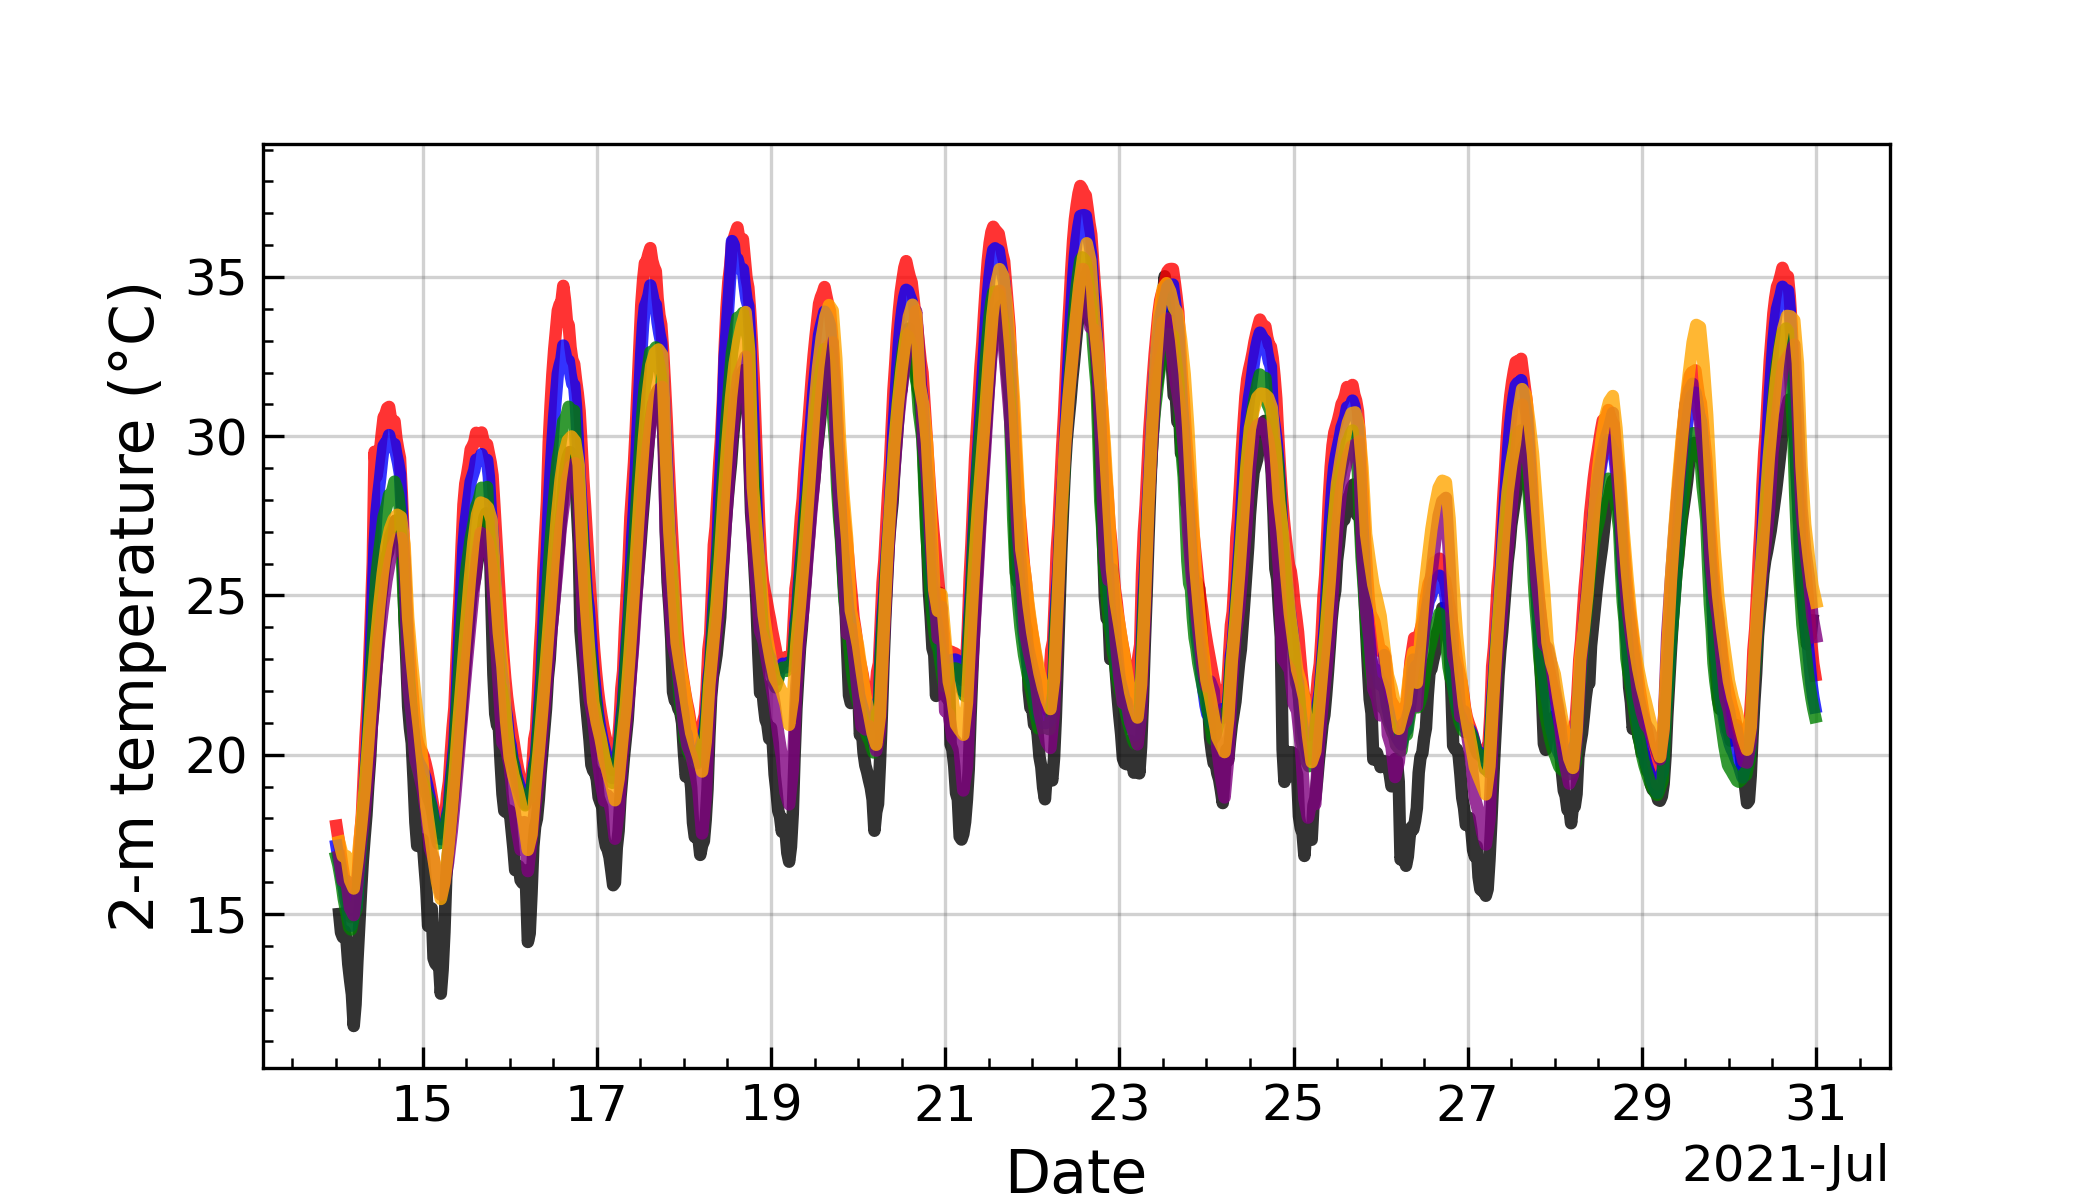
\includegraphics[width=\textwidth]{images/chap5/time_series_cendrosa_t2m.png}
        \end{subfigure} &
        \begin{subfigure}[t]{0.5\textwidth}
            \caption{}
            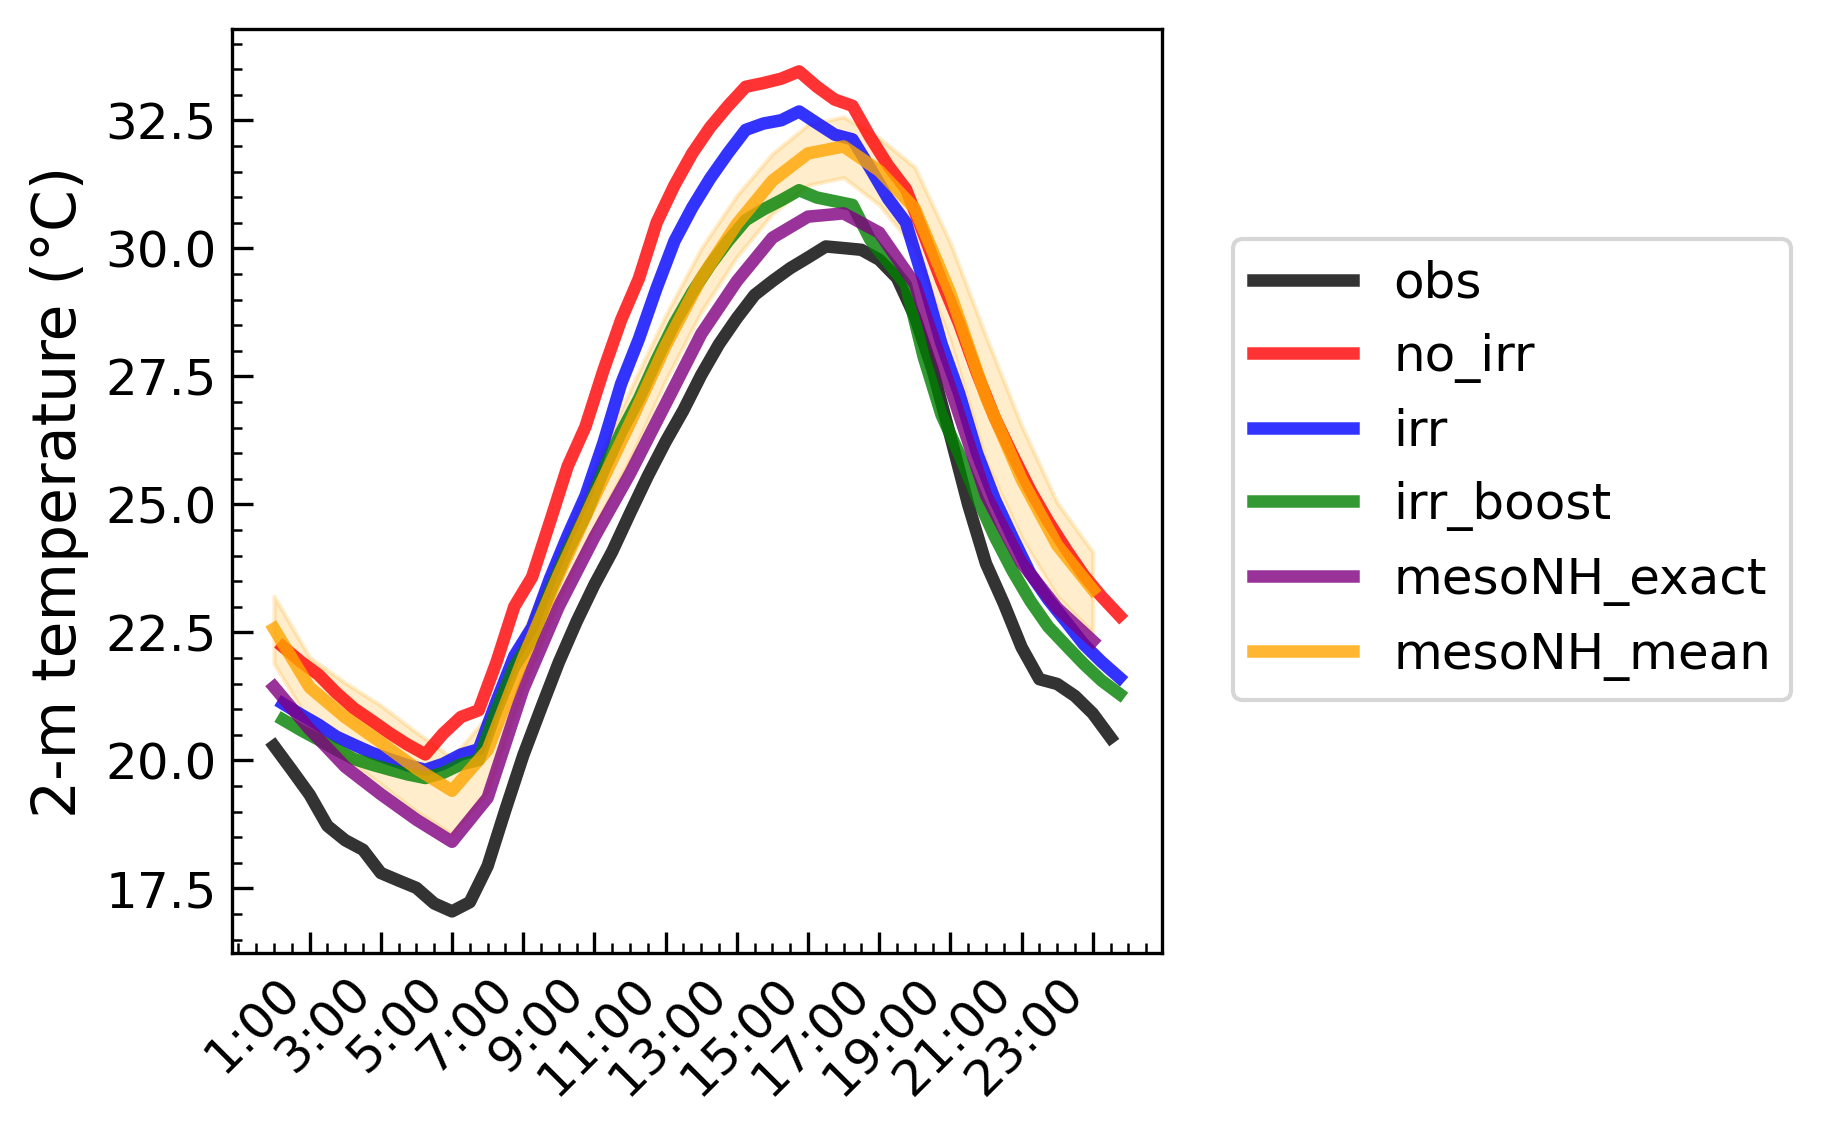
\includegraphics[width=\textwidth]{images/chap5/diurnal_cycle_cendrosa_t2m.png}
        \end{subfigure} \\
        
        \vspace{1em} % Add vertical space between the rows

        \begin{subfigure}[t]{0.5\textwidth}
            \caption{}
            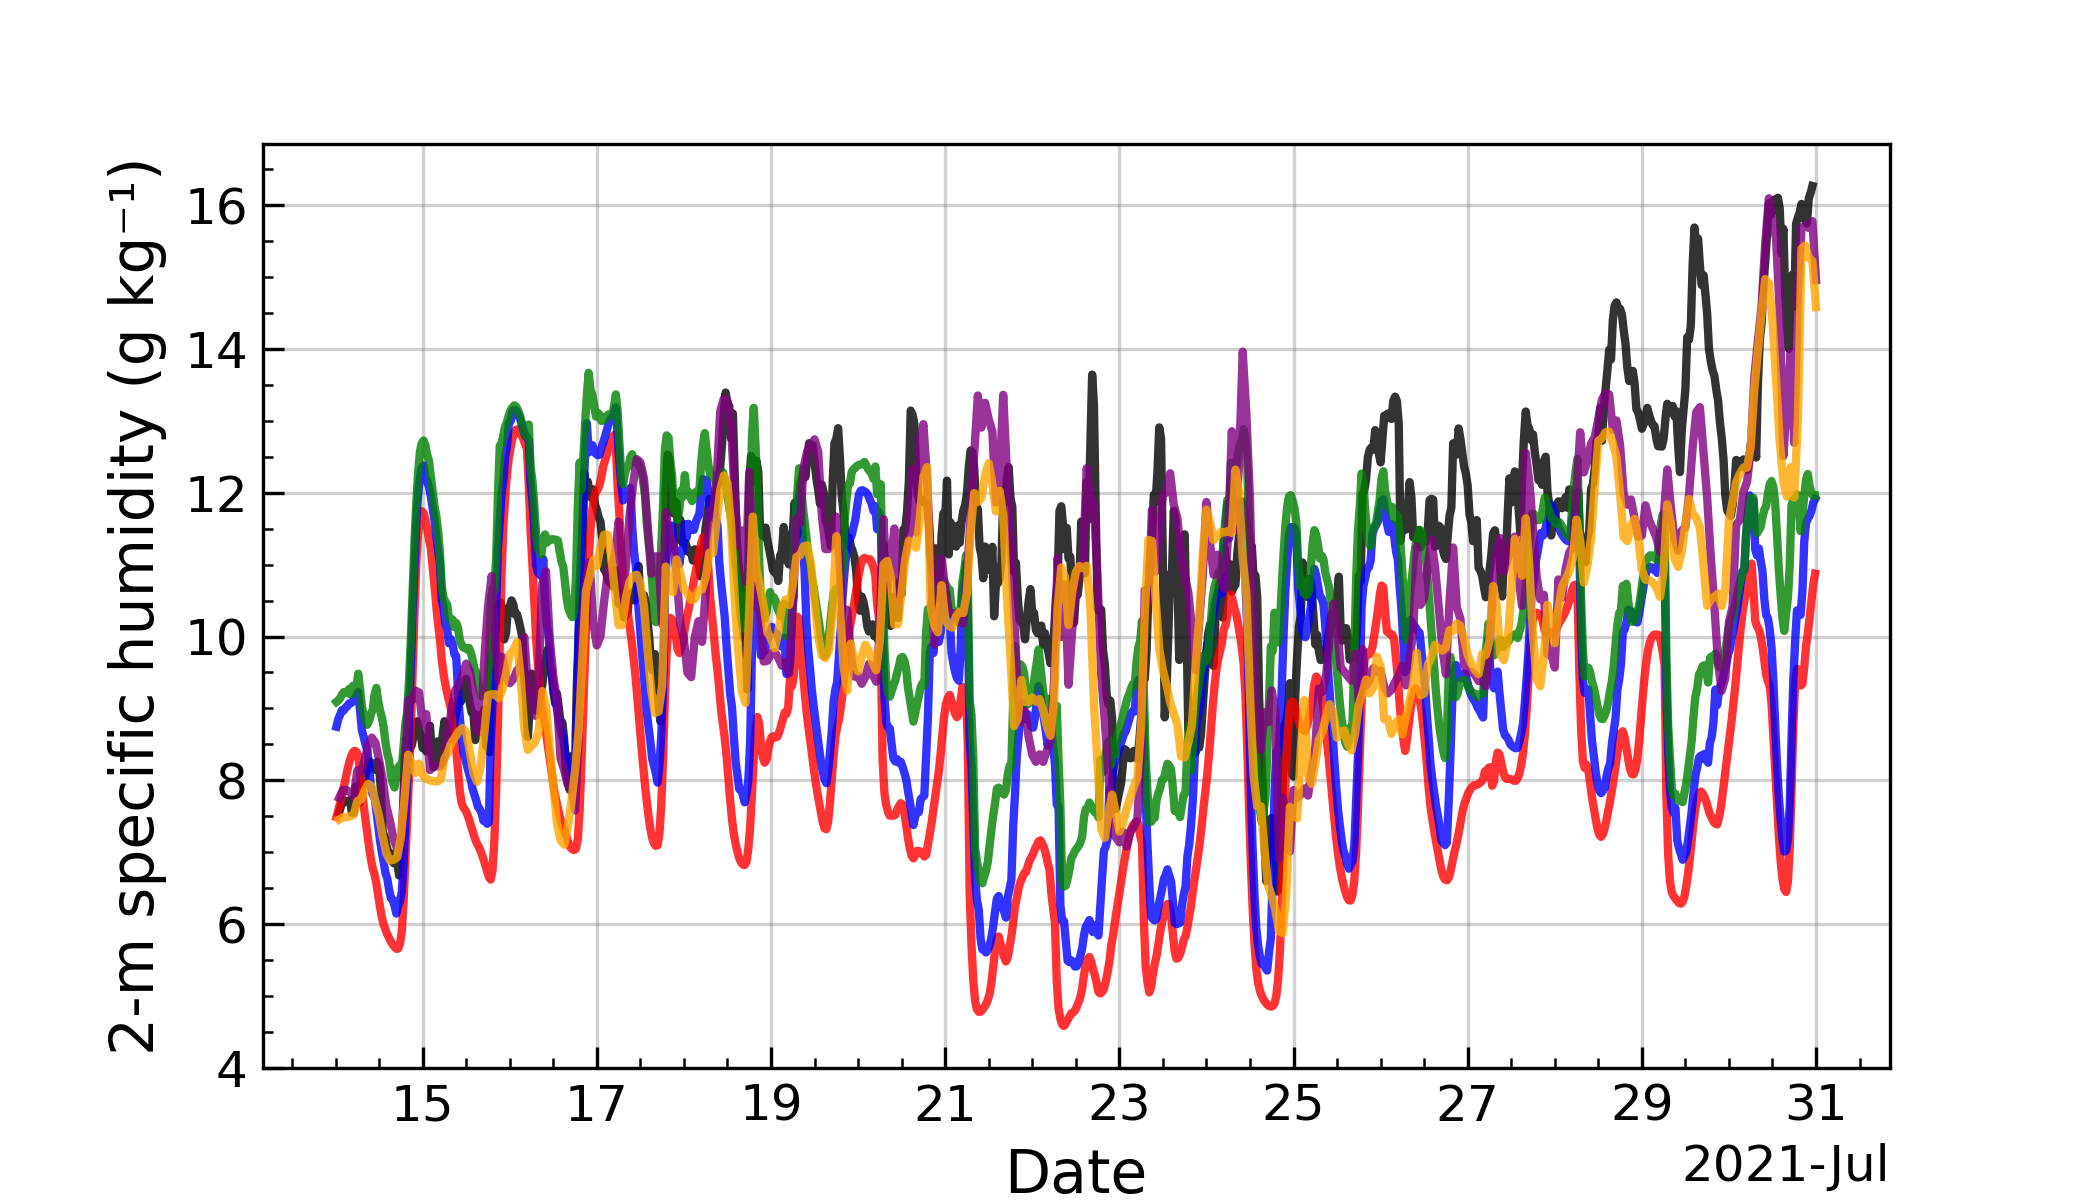
\includegraphics[width=\textwidth]{images/chap5/time_series_cendrosa_q2m.png}
        \end{subfigure} &
        \begin{subfigure}[t]{0.5\textwidth}
            \caption{}
            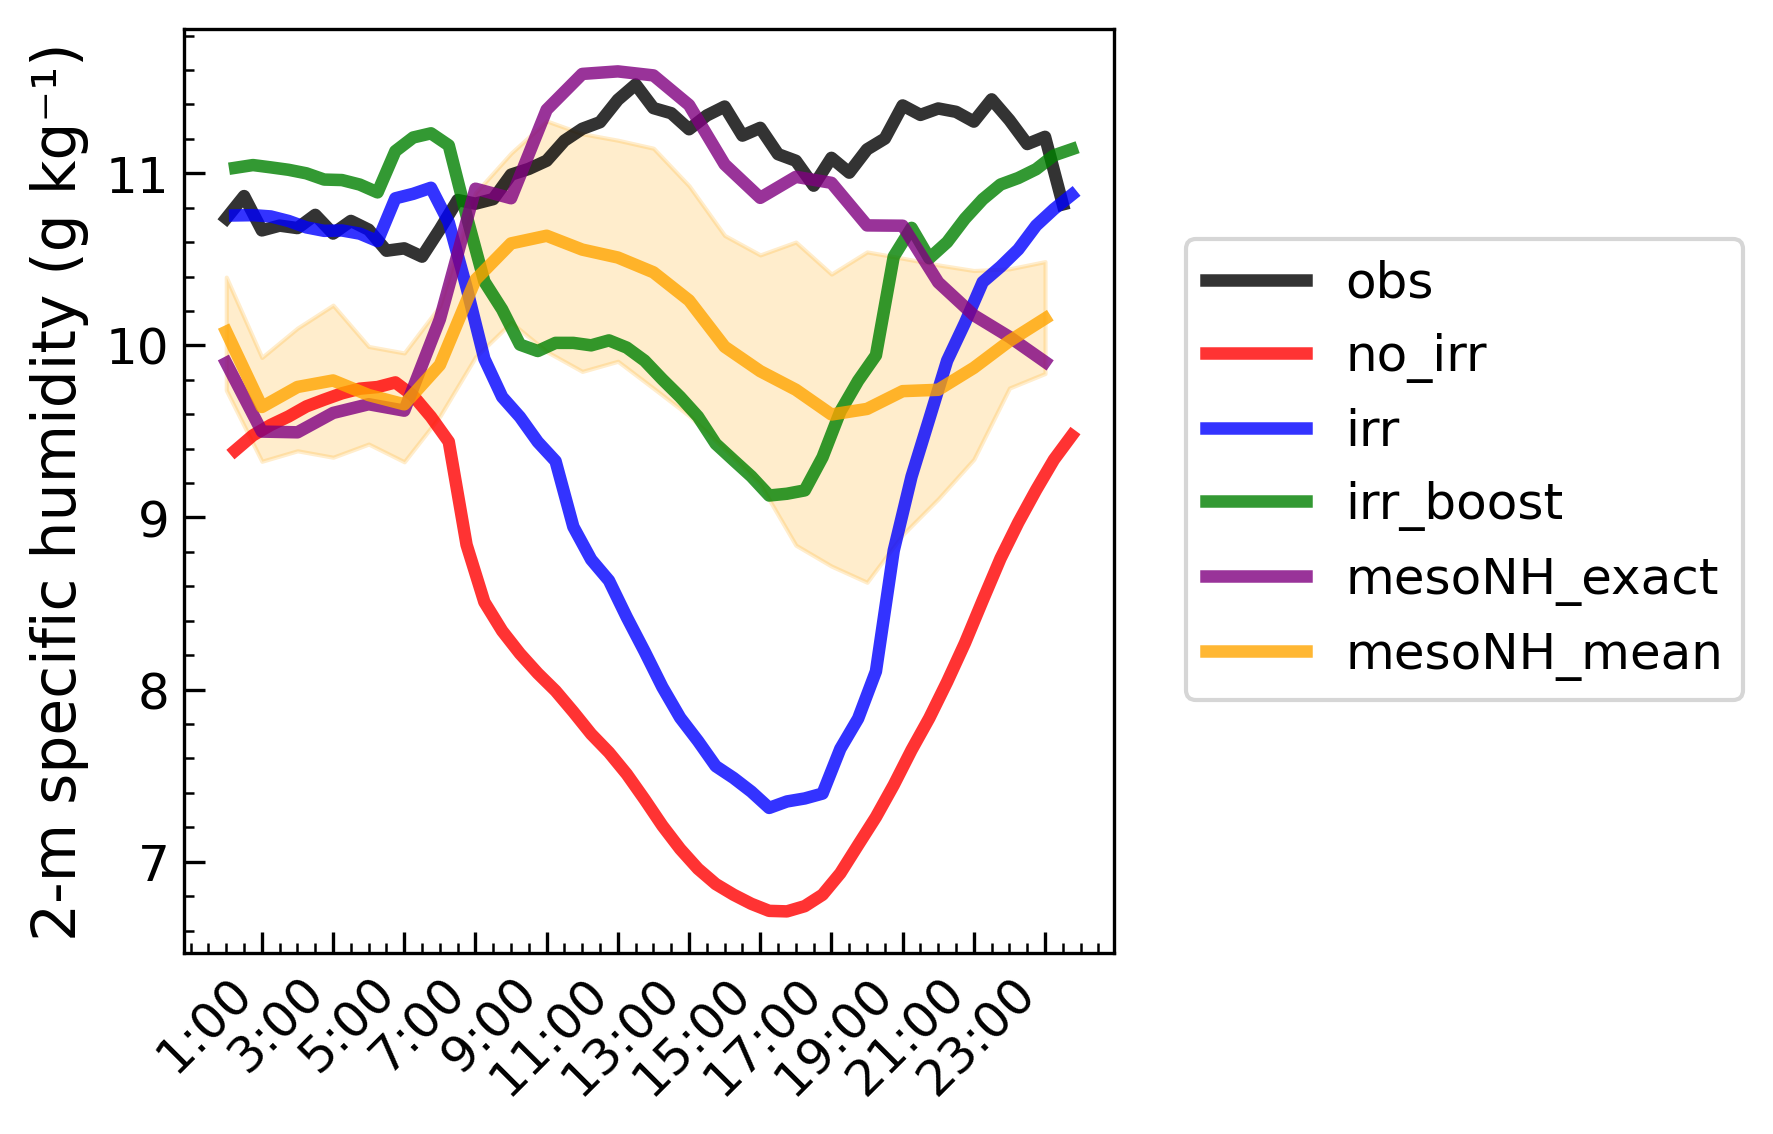
\includegraphics[width=\textwidth]{images/chap5/diurnal_cycle_cendrosa_q2m.png}
        \end{subfigure} \\
    \end{tabular}
    \caption{Time series and mean diurnal cycle of 2-m temperature and specific humidity at La Cendrosa (irrigated site), July 15-31 2021.}
\end{figure}

%Els Plans t2, q2m
\begin{figure}[hbtp]
    \centering
    \begin{tabular}{cc}
        \begin{subfigure}[t]{0.5\textwidth}
            \caption{}
            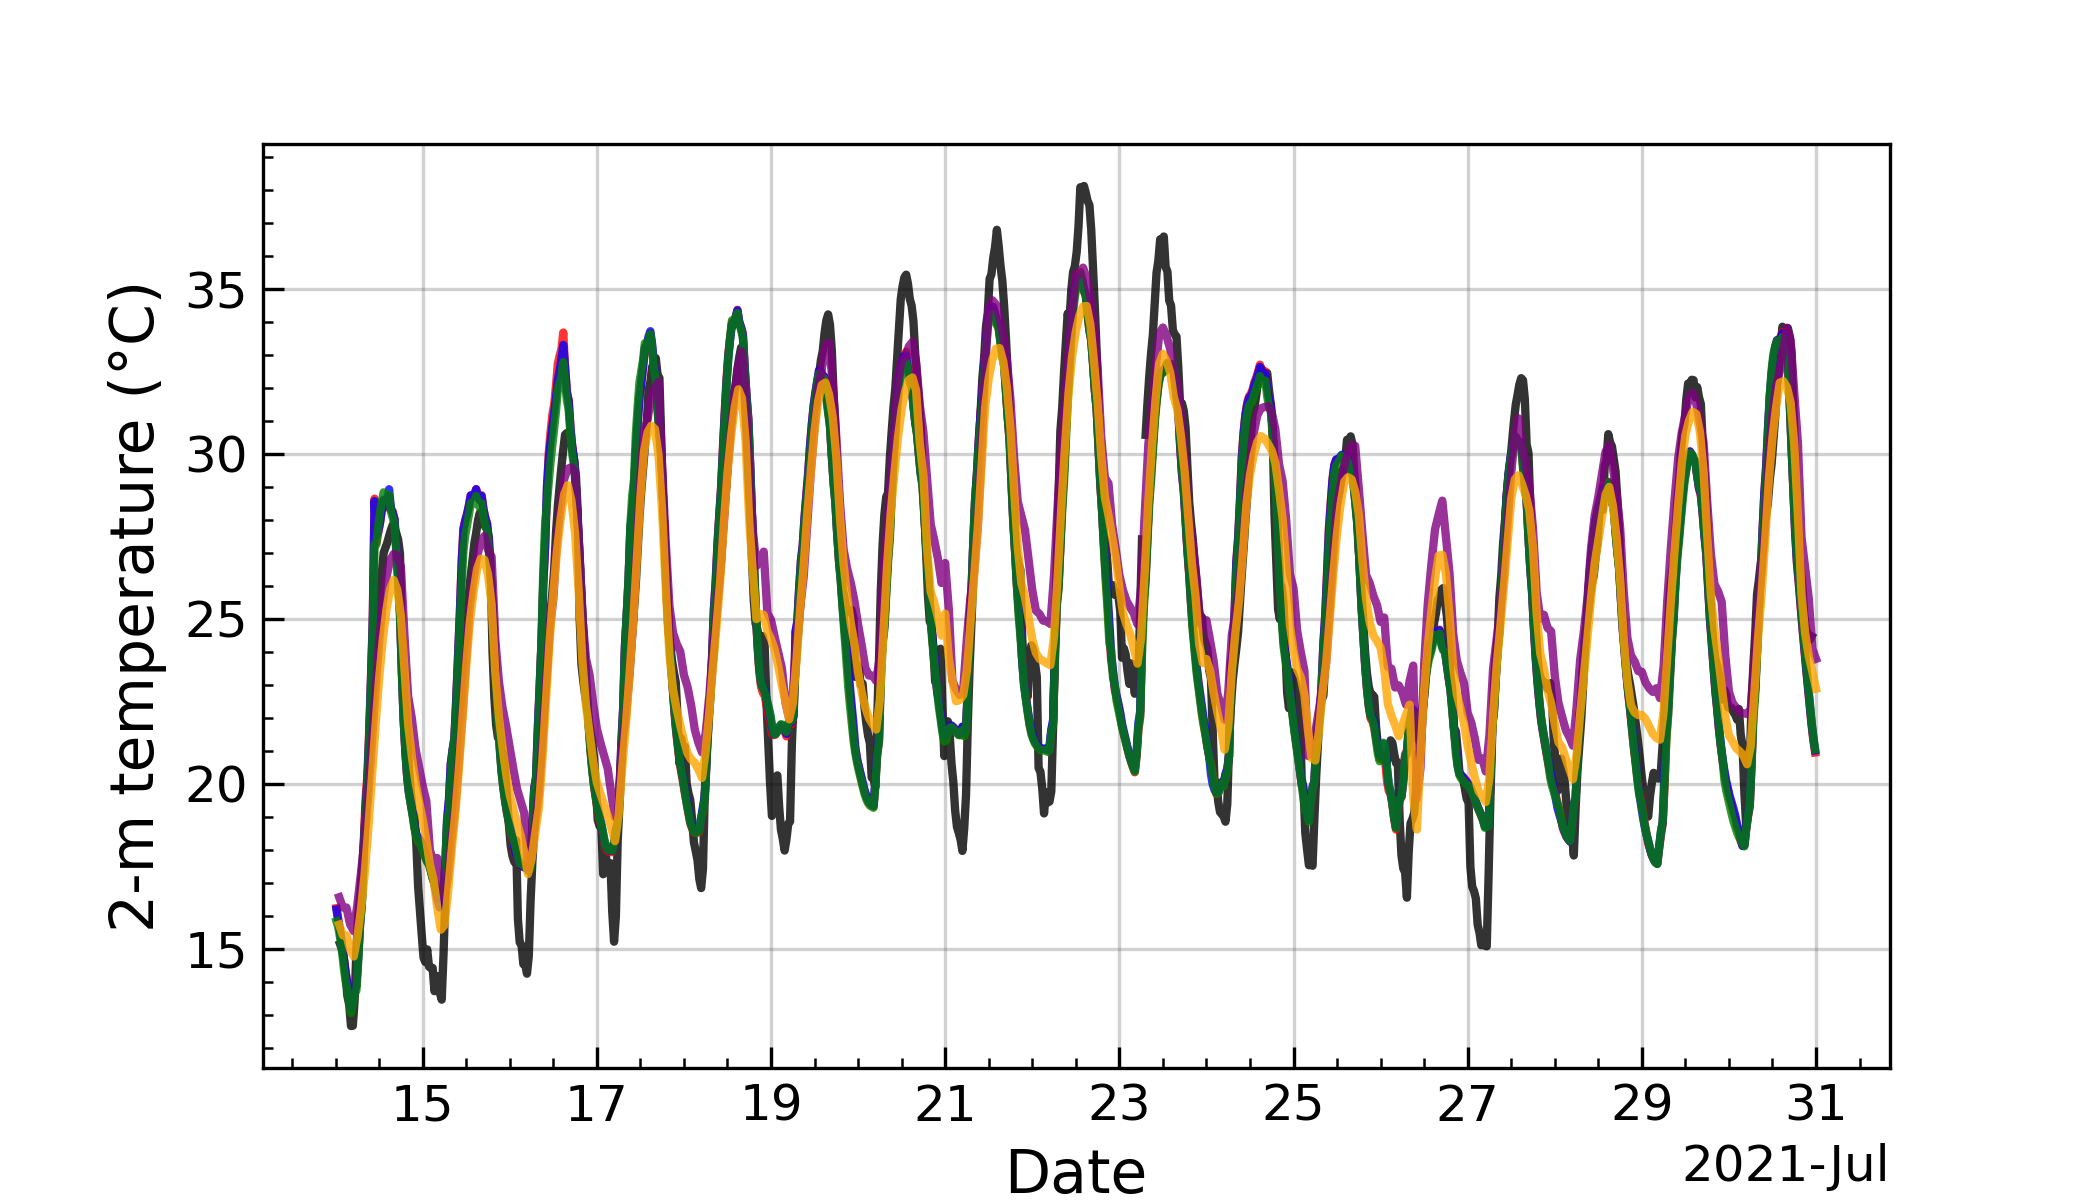
\includegraphics[width=\textwidth]{images/chap5/time_series_elsplans_t2m.png}
        \end{subfigure} &
        \begin{subfigure}[t]{0.5\textwidth}
            \caption{}
            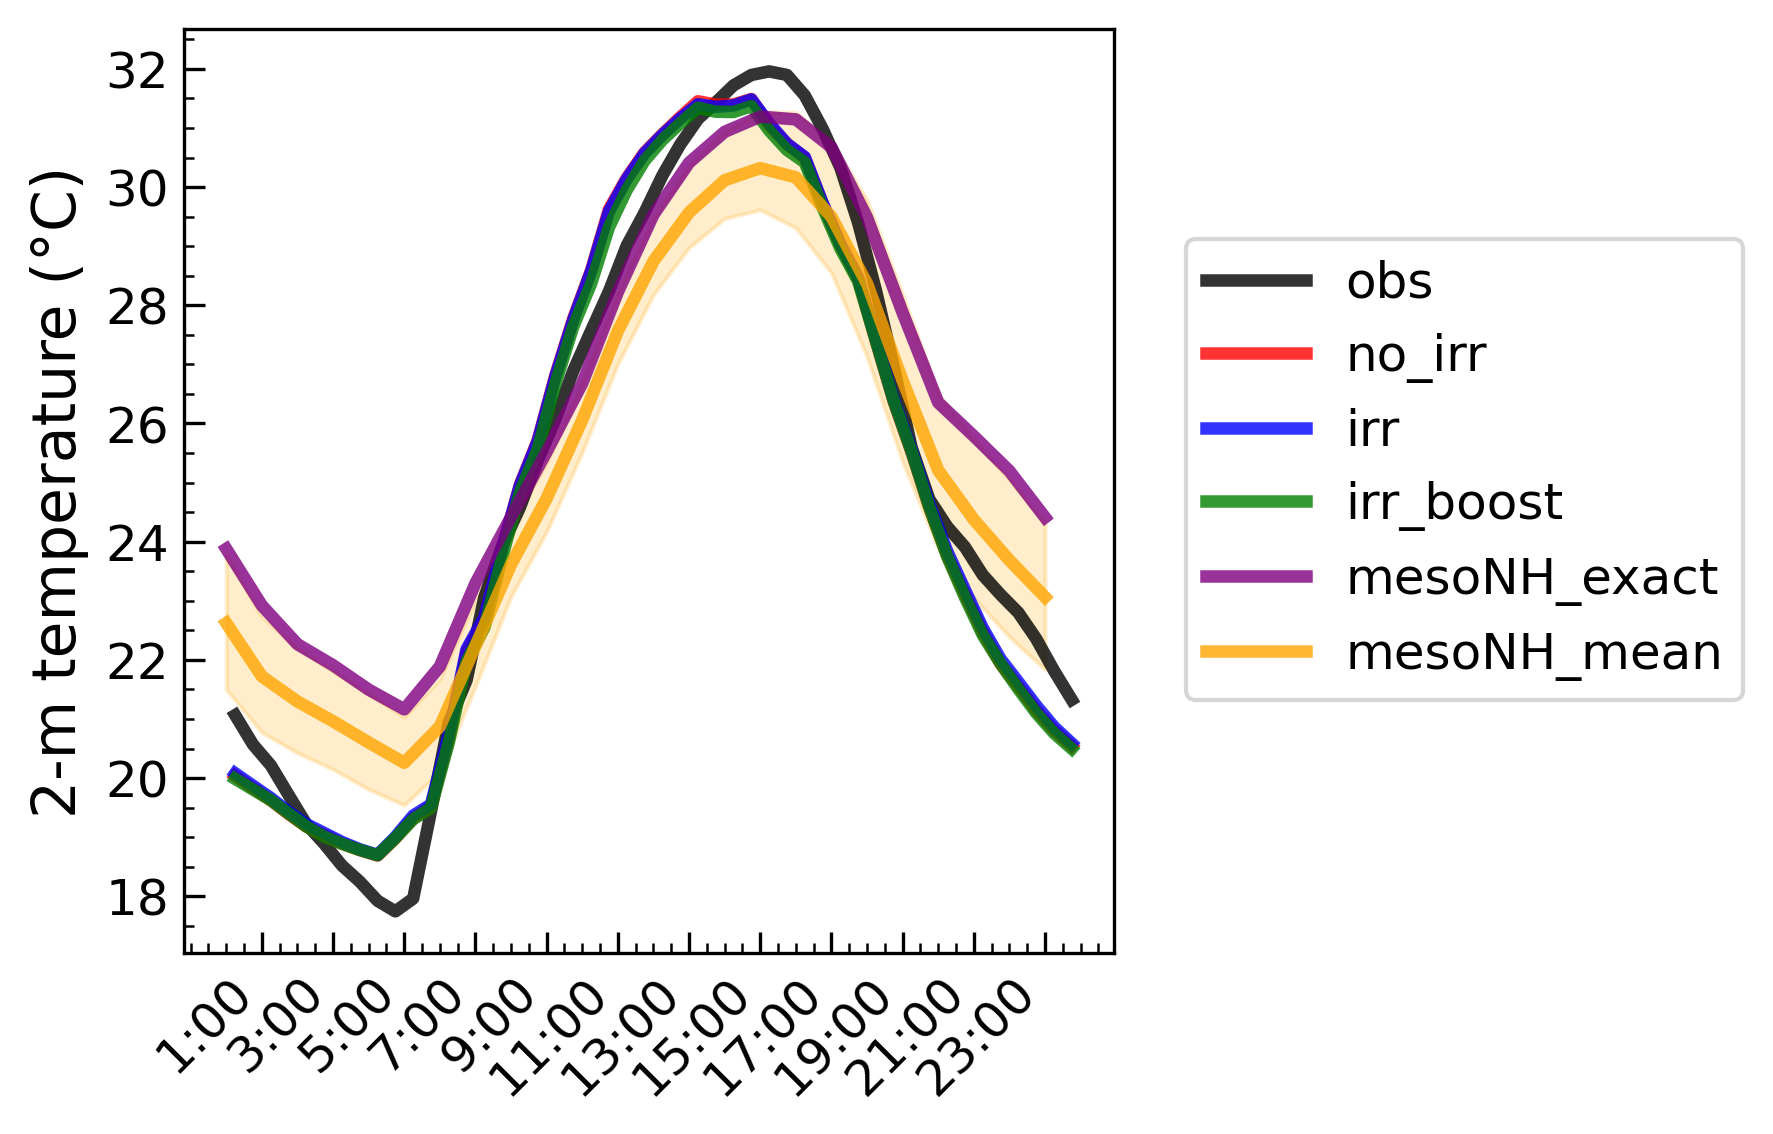
\includegraphics[width=\textwidth]{images/chap5/diurnal_cycle_elsplans_t2m.png}
        \end{subfigure} \\
        
        \vspace{1em} % Add vertical space between the rows

        \begin{subfigure}[t]{0.5\textwidth}
            \caption{}
            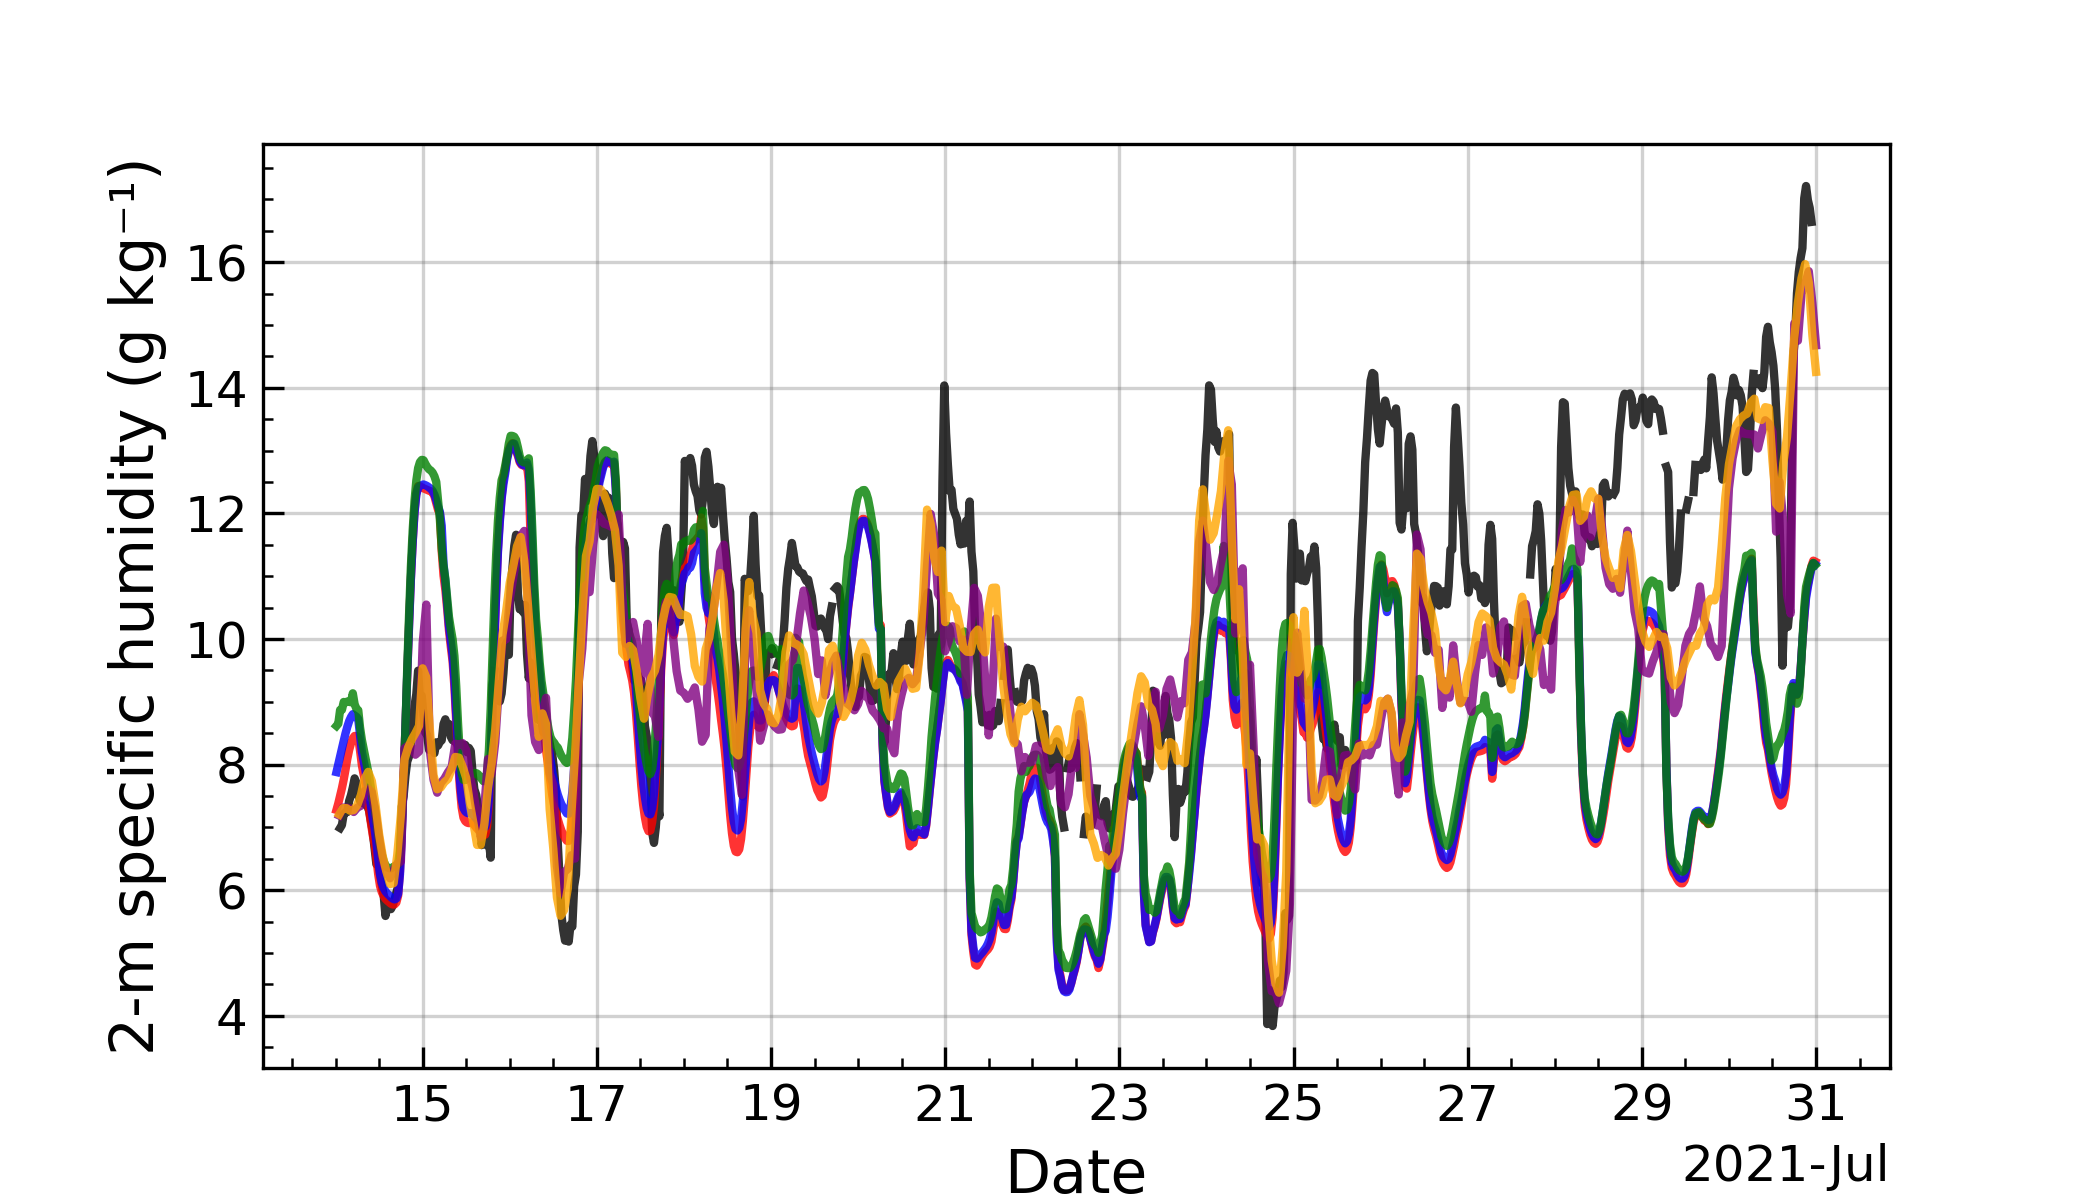
\includegraphics[width=\textwidth]{images/chap5/time_series_elsplans_q2m.png}
        \end{subfigure} &
        \begin{subfigure}[t]{0.5\textwidth}
            \caption{}
            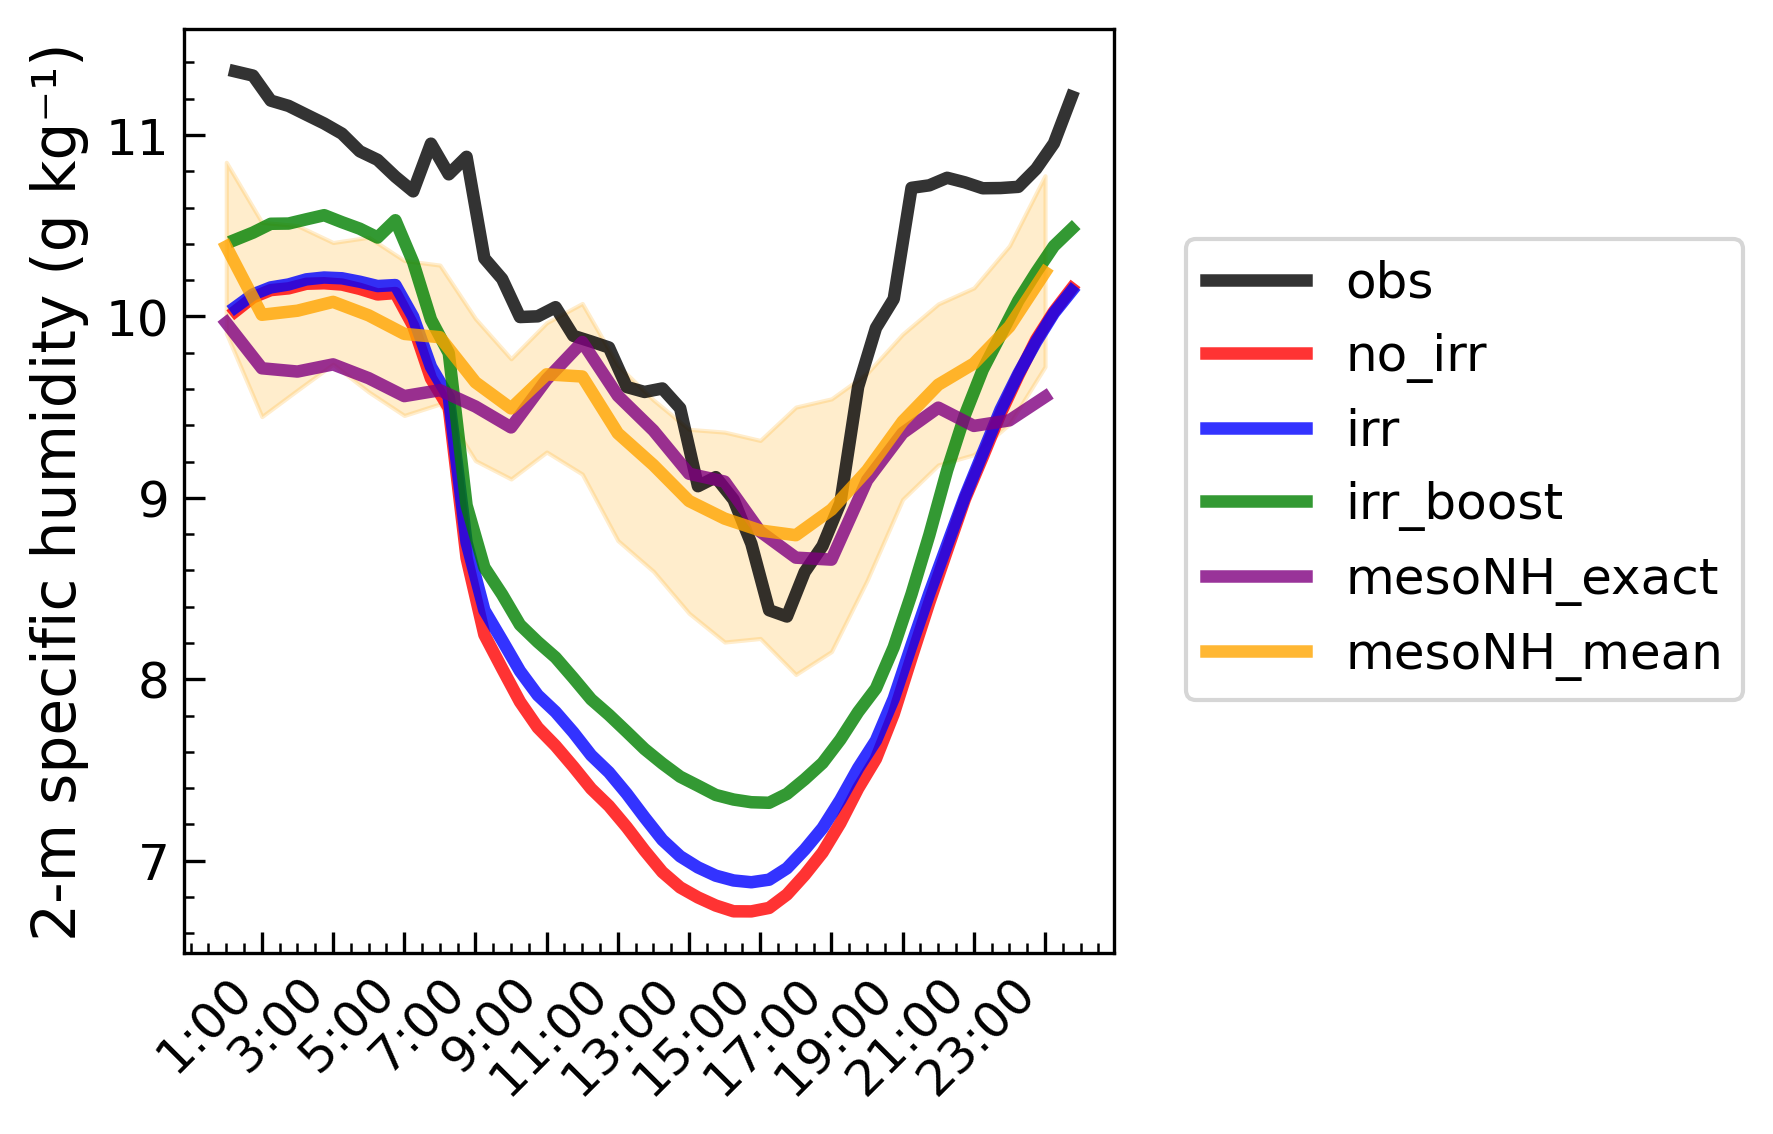
\includegraphics[width=\textwidth]{images/chap5/diurnal_cycle_elsplans_q2m.png}
        \end{subfigure} \\
    \end{tabular}
    \caption{Time series and mean diurnal cycle of 2-m temperature and specific humidity at Els Plans (rainfed site), July 15-31 2021.}
\end{figure}

\clearpage

\section{Vertical structure of the atmosphere}

\clearpage

\section{Chapter conclusions}